% !TEX program = pdflatexmk

% The line above is a directive for TeXShop and TeXworks.
% - For TeXShop: this directive enables one-click typesetting for this file, 
% 	instead of the multi-step process usually needed for BibTeX.
% - For TeXworks: the directive will only work after TeXworks has been 
% 	configured to use latexmk; see 
% <https://github.com/TeXworks/texworks/wiki/AdvancedTypesettingTools> 

\documentclass[11pt]{amsart}

\usepackage[letterpaper,left=125pt,right=125pt]{geometry}

% ^^^^^^^^^^^^^^^^^^^^^^^^^^^^^^^^^^^^^^^^^^^^^^^^^^^^^^^^^^^^^^^^^
% DO NOT change anything above this line! 
% (We need standard margins and type size.)
% In particular, don't include your own "geometry" settings further down.



%%%%%%%%%%%%%%%%%%%%%%%%%%%%%%%%%%%%%%%%%%%%%
% The following part of the preamble sets up packages, theorems, and shortcuts; 
% you can edit it, but you won't need to change much.

%% Load Packages:

\usepackage[english]{babel}
\usepackage {amsmath}  % provides lots--- e.g. equations, matrices, definition by cases
\usepackage{amssymb}  % provides common mathematical symbols
\usepackage{amsfonts}
\usepackage{amsthm}     %provides \newtheorem, \theoremstyle, \begin{proof}...\end{proof}
\usepackage{graphicx}  % allows importation of graphics files
\usepackage{float}
\usepackage[colorlinks,linkcolor=blue,citecolor=blue,urlcolor=blue]{hyperref} % typesets URLs and clickable cross-references and links
%\usepackage{hyperref} % if you don't want colored links, just use the simpler command

%% Bibliography support
\usepackage[backend=biber,isbn=false,url=false]{biblatex} 
% notes on settings:
% backend=biber: we are using the newer tool biber for processing (rather than the older bibtex program)
% isbn=false, because printing ISBNs is distracting clutter
% urls=false: we don't need to show URLs for primarily print sources (distracting); 
%							this setting does *not* apply to `@online` records 
\usepackage{multirow,array}
\addbibresource{refs.bib} % CHANGE this to the name of your BibTeX database file (see instructions below)


%% Environments for theorems, etc.. 

% You can add your own theorem-like environments, see https://en.wikibooks.org/wiki/LaTeX/Theorems
% The basic formats are 
% \newtheorem{name}{display-text}[numbered-within]  and
% \newtheorem{name}[numbered-like]{display-text}

\newtheorem{thm}{Theorem}[section] %\newtheorem{name}{display-text}[numbered-within]

\newtheorem{lem}[thm]{Lemma} %\newtheorem{name}[numbered-like]{display-text}
\newtheorem{cor}[thm]{Corollary}
\newtheorem{prop}[thm]{Proposition}
\newtheorem{alg}[thm]{Algorithm}

% the batch of theorem-like environments above are typeset in the default "plain" style, with italic text

\theoremstyle{definition}                  % switch to a different style: roman text and extra spacing above and below
\newtheorem{defn}[thm]{Definition}
\newtheorem{conj}[thm]{Conjecture}
\newtheorem{prob}[thm]{Problem}

\theoremstyle{remark}                       % switch to yet another style: roman text, no extra spacing
\newtheorem{exmp}[thm]{Example}  
\newtheorem{rem}[thm]{Remark}
\newtheorem{claim}[thm]{Claim}  

%% If you use numbered equations in a long document, it is preferred to number
% as (x.y), where x is section number, y is equation number

\numberwithin{equation}{section}


%% Common typesetting for common mathematical objects

\newcommand{\R}{\mathbb{R}}
\newcommand{\Q}{\mathbb{Q}}
\newcommand{\N}{\mathbb{N}}
\newcommand{\Z}{\mathbb{Z}}
\DeclareMathOperator{\rank}{rank}
\DeclareMathOperator{\dimension}{dim}



%%%%%%%%%%%%%%%%%%%%%%%%%%%%%%%%%%%%%%
% BEGIN: You'll _need_ to edit everything below....


%  Your data for title, author, etc.

\title{Algorithmic Transit Optimization: Evolutionary Algorithms Applied} % here, the command format is  \title[Abbreviated Title for Header]{Full Title}. But if your title is short, simply use \title{Full Title}
\thanks{This document is a senior thesis submitted to the Department of Mathematics and Statistics at Haverford College in partial fulfillment of the requirements for a major in Mathematics.} % REQUIRED: don't change this line
\author{Harrison Weinstock}
\date{\today} % don't forget to update the date!

\begin{document}

\begin{abstract} % REQUIRED (and needs to go before \maketitle)
This project leverages artificial intelligence techniques from the field of evolutionary computing to investigate the task of optimizing the geometry of urban transit systems. Working with the San Francisco Municipal Transportation Agency (SFMTA) bus network, we attempt to optimize the shape and organization of the routes using a custom genetic algorithm (GA). Due to the complexity of the problem, multiple iterations of the model are proposed to incorporate new ideas, and address shortcomings in previous versions. The results exemplify both the GAs ability to consistently find unexpected ways to maximize its fitness function and the nuanced complexities in the problem of transit optimization. 
\end{abstract}

\maketitle % Actually typeset the title, author, etc.


\tableofcontents % OPTIONAL. See https://en.wikibooks.org/wiki/LaTeX/Document_Structure#Table_of_contents for more information.

%%-------------------------------------------------------------------------------------------------
\section{Introduction}

\subsection{Urban Public Transit Optimization}
    For the scope of this paper, we will refer to transit systems in place of urban public transit systems. It is also important to highlight that the optimization of said transit systems can hold many different meanings depending on the perspective of the reader. To consider a few perspectives, consider the economic point of view, where the ideal transit system efficiently uses funds and labor to maximize the profit margin between system costs and system profit. Alternatively, consider the perspective where a transit system is about maximizing access especially to those who require the subsidized mobility the most. Finally, consider an architectural view, where an effective transit system contributes to the city structure and aesthetic. Therefore, there is no single answer to what an optimized public transit system looks like \cite{walker2012, litman2011}.

    The multitude of perspectives on the goal of transit highlights an issue any transit system must address with critical importance: everyone has a different relationship with the transit system and wants different functionalities from it. When trying to please the economist to develop a financially efficient system, one might upset the social worker and make sacrifices to which neighborhoods receive the most route coverage. While many conflicts arise in trying to please all parties, two of the most central are the trade offs between maximizing ridership or coverage, as well as maximizing user costs or operator costs. 

    \subsubsection{Coverage versus Ridership}
    To illustrate the trade-off, consider the extreme example of transit design in the New York City area. If we want to optimize ridership, we could run as many services within Manhattan, the densest area of the city, as possible. We would run these services at the cost of not running other services that serve less densely populated areas such as Long Island or Westchester. While our trains in Manhattan would be carrying more people per service than those in suburban areas, we have now lost a degree of coverage.

    There is no correct solution to this problem, but rather a decision that must be made in terms of allocating resources to maximize ridership or coverage. Therefore, when phrasing the question of optimizing public transit, we must be more specific in what we are optimizing. 

    \subsubsection{User Costs versus Operator Costs}
    Unfortunately, ridership and coverage is not the only example of conflicting objectives when designing transit. Finding a balance of minimizing both user costs and operator costs poses an additional challenge. We can define user costs as the amount of time a person must spend to get to their destination. We can then define operator costs as the amount of resources used to operate and maintain the network. Notice that when considering one of the two in isolation, the other may be negatively affected. For example, we can reduce the user cost by doubling the frequency of services run for each route, but this would have the potential to double the fleet size necessary for each route, drastically increasing the operator costs. 

    Due to the conflicting objectives involved in transit optimization, the problem of evaluating a system's performance in a general manner is extremely complicated. 
    Specifically, this type of problem is called \textit{Multi-objective optimization}, meaning an optimization problem concerning multiple objectives concurrently \cite{arbex2015}. One method of handling multiple objectives is to optimize a single function while the others remain fixed. In the example of considering both user costs and operator costs, Jha and Schonfeld optimize a specific transit route design by setting a maximum budget the operator can spend, then minimizing user costs under that budget \cite{jha2007}. Such a method can be useful when one of the quantities being optimized can instead be viewed as a constraint, as is in this case with budget. In contrast, trying to optimize both user costs and operator costs simultaneously has also been investigated by Arbex who uses a dynamic objective function that switches between minimizing user costs and minimizing operator costs on each round of an iterative optimization process \cite{arbex2015}. 

    \subsubsection{Designing a System}
    We can describe the design of a transit system as a combination of $3$ interdependent problems \cite{arbex2015}:
    \begin{itemize}
        \item \textbf{Network geometry:} the structure of the routes themselves describing where routes stop and how they move between stops. 
        \item \textbf{Frequency Assignment and Timetable Development:} an assignment of frequency to each route in the network. This answers the question of how often each trip stops at any given stop and determines the expected wait time for different routes \cite{cevallos2006, hu2005}. 
        \item \textbf{Fleet and Crew Scheduling: } the allocation of units to different routes in the network as well as the scheduling of driver shifts to accommodate the time table as well as respect labor laws. 
    \end{itemize}
    Typically these problems are solved in the order presented since each problem is highly affected by the answer to those above it in this list. However, that is not to say that the opposite is not also true and that for example fleet and crew scheduling ability does not affect frequency and timetable development. Notice that no piece of the system directly follows from previous implementations since each stage requires a new constraint or problem to tackle. 

    Because each problem listed above involves high degrees of complexity, this paper will focus on the geometry problem and specifically the construction of the routes. The specific formulation of the problem will be done once we review the tools we will use: evolutionary computing and specifically genetic algorithms.  
    
\subsection{Evolutionary Computing: Genetic Algorithms}

\subsubsection{Building Blocks of Genetic Algorithms (GAs)}

    GAs are an evolutionary computing technique taking inspiration from natural evolutionary processes \cite{mitchell1998}. 
    The outline of a generic GA is as follows:
    \begin{itemize}
        \item Determine an \textbf{encoding} scheme so that we can represent solutions to the problem we are trying to optimize in a concrete way. 
        \item Initialize some population $P$ of potential solutions in encoded form, often involving randomly generating some or all. 
        \item For each member $p_i \in P$, evaluate it with respect to some \textbf{fitness function} $f$. 
        \item Using these evaluations, create a new population $P'$ using techniques such as \textbf{selection}, \textbf{crossover}, and \textbf{mutation}. 
        \item Run the algorithm again, starting with $P'$, and repeat until desired performance is observed. 
    \end{itemize}

    \begin{figure}
     \begin{center}
         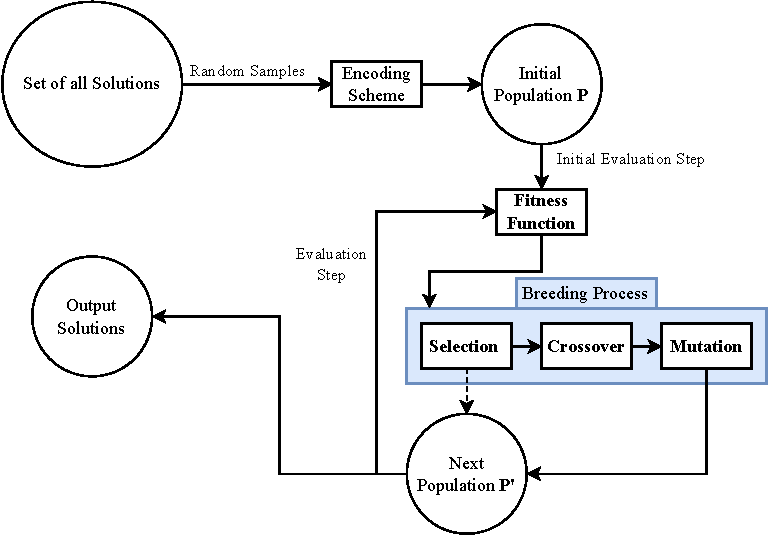
\includegraphics{Thesis/diagrams/general_ga.pdf}
     \end{center}
    \caption{General GA process}
     \label{diagram:GA}
     \end{figure}
    Refer to Figure \ref{diagram:GA} for a visual representation of the algorithm. Notice that each circle in this figure represents a set, whereas each rectangle represents a function. The breeding process is a specific piece of the GA that refers to the collection of techniques used to generate the next population. Additionally, the dotted line in the figure is there to represent a common technique in GAs called \textit{elitism}, where the best performing solutions are carried into the next population \cite{mitchell1998, nayeem2014}.

\subsubsection{GA Applied to Prisoner's Dilemma}
The prisoner's dilemma is a two player game where each player independently chooses to either confess or remain silent. Depending on how each player answers, they each receive a sentence of a certain length. Let $A$ be our first player and $B$ be our second. We represent the outcomes of the game in Table \ref{tab:PD} where the entry $(a, b)$ in the table represents the case where $A$ receives a sentence of $a$ years and $B$ receives a sentence of $b$ years. 
\begin{table}[h]
\begin{center}

    \setlength{\extrarowheight}{2pt}
    \begin{tabular}{*{4}{c|}}
      \multicolumn{2}{c}{} & \multicolumn{2}{c}{Player $A$}\\\cline{3-4}
      \multicolumn{1}{c}{} &  & Stay Silent  & Confess \\\cline{2-4}
      \multirow{2}*{Player $B$}  & Stay Silent & $(1,1)$ & $(3,0)$ \\\cline{2-4}
      & Confess & $(0,3)$ & $(2,2)$ \\\cline{2-4}
    \end{tabular}
    \end{center}
    \caption{\label{tab:PD} Prisoner's Dilemma}
\end{table}

Consider repeating this game multiple times so that each participant is aware of the outcomes in previous iterations. We then define each player's score as the total sentence they accumulate across all the rounds. Now, we can phrase our example problem as the following:
\textit{If the previous $3$ rounds' outcomes are known, what is the optimal move in the following round to minimize my total score?}
The first step in solving this problem with a GA is to determine a proper encoding of a strategy. We are looking at the past $3$ rounds, where each round has $4$ potential outcomes. Thus, there are $64$ possible states from the previous $3$ rounds. If we enumerate these cases $s_0, \ldots, s_{63}$ we can represent a strategy as a 64-bit binary number where a $1$ in position $i$ corresponds to confessing when the past $3$ rounds fall under case $i$ \cite{holland1992}. Note that many other possible encoding schemes exist that could allow for non-deterministic strategies, where the strategy is not fixed based on the state and instead involves some randomness. However, the outlined encoding is effective in representing all strategies that don't involve any randomness concisely. 

Now, we define our fitness function. In order to evaluate the effectiveness of a strategy, we can create random pairings of strategies and have them play the prisoners dilemma game for a single round, with a randomized state for the previous $3$ rounds.

More formally, let $M \in \mathbb{N}$ be some parameter and form random pairs of the strategies in the populations such that each member of the population occurs in exactly $M$ pairs. Now, for each pair, have the two strategies face off against each other in a single round with a randomized state. Then, for any strategy, assign it a fitness equal to the inverse of its average score across all match-ups it participated in. This method of fitness assignment is closely related to the idea of tournament selection \cite{mitchell1998}. 

Note that we want to invert this average score because that allows us to maintain the intuition that high fitness means a low score and thus high performance. 

Now, we have a few more pieces to define before we can plug this algorithm into the template from earlier. 

First, we can implement a straightforward elitist selection where we take the top performing $c$ percent, where $c$ is some parameter, and copy them into the next population $P'$ \cite{mitchell1998}.

Next, we want to define a crossover strategy. Crossover can be thought of as 'breeding' solutions to create new ones. For a simple strategy, we can implement \textit{single-point crossover} with a straightforward selection process. We randomly select two parents $p_1, p_2$ from the top $c$ percent where strategies that achieve a higher fitness function value have a higher probability of being selected as a parent. Then, we uniformly sample an index from $\{0, \ldots, 63\}$. Then, we define two children $c_1$ and $c_2$ such that $c_1$ is equal to the string $p_1$ up to index $i$ concatenated with $p_2$ after index $i$. We can define $c_2$ similarly by starting with $p_2$ up to index $i$ and $p_1$ after index $i$ \cite{holland1992}. A visual representation of this idea can be found in Figure \ref{fig:singlePointCrossover}. 

\begin{figure}[H]
    \centering
    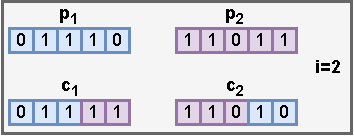
\includegraphics{Thesis/diagrams/crossover_example.pdf}
    \caption{Single point crossover}
    \label{fig:singlePointCrossover}
\end{figure}

Finally, only one operation remains to be defined: mutation. As a simple approach to mutation, we can flip each bit of the children with probability $r$, where $r \in (0, 1)$ is some universal parameter that remains constant. 

Now, we can plug all of these pieces into the template above and we have constructed our first GA. 

Using a similar construction of the GA, Axelrod and Forrest analyzed the Prisoner's Dilemma problem and were able to observe a 'bluffing' strategy develop within the top performing members of later generations \cite{axelrod1987, holland1992}. That is, the strategy would start by staying silent such that the other player was more likely to stay silent as well, then swap to confessing in order to minimize their score and therefore maximize their fitness. 

\subsubsection{More Terminology and General Techniques}
When working with GAs, it is common to abstract away the actual solution being computed and instead focus on the encoding the algorithms is working with. Borrowing terms from biology, an encoded solution is commonly referred to as a \textit{chromosome}. Therefore, we can think of encoding schemes as functions that map solutions to the the chromosome space. Within a chromosome, there are many places for differences to occur. Each of these locations is commonly referred to as \textit{genes} and their values as \textit{alleles} \cite{jha2007}. For example, if we consider the example from the prisoner's dilemma, the 64-bit string is the chromosome, the 64 indices are the genes, and the $1$ or $0$ at each index is an allele. 

Using this terminology can make it easier to talk about the development of the population without referring to any specifics of the encoding scheme. Additionally, it makes the explanation of the ``messy'' GA, a term coined by David Goldberg, more intuitive \cite{goldberg1989}. 

A \textit{messy GA}, is a variant of GAs that does not operate under the same restrictions. In the standard model, we are computing on single chromosomes of a fixed size. However, in the messy approach, the size and number of chromosomes is allowed to vary \cite{goldberg1989}. The intuition for this approach is the problem can be reduced to easier sub-problems such that each chromosome becomes highly effective in handling a specific sub-problem, then combining them can create a solution able to solve many of the smaller problems and therefore the larger problem. 

In the example of transit systems, a sub-problem could be the optimization of an individual route, or the optimal transit service for a particular area of a city. Another example could be the optimization of the bus lines, rail lines, and ferry services independently.

However, the implementation of messy algorithms becomes more complicated since standard operations within the GA assume equal size chromosomes. Therefore, the implementation is often done in two stages: a \textit{primordial phase} and a \textit{juxtapositions phase}, the former being the optimization of each unit or the solution to each sub-problem, and the latter being the optimization of their combinations \cite{mitchell1998}. 

Continuing with the example of transit systems, the juxtaposition phase could mean combining different 'optimal' routes or pieces of a transit system together to optimize the overall network. 

Using these tools, we can begin to formalize our genetic algorithm for the transit system optimization problem. 

\section{Procedure: Defining the Problem}
\subsection{Problem Formulation}
We are investigating the optimization of transit network geometry. We will assume the existing network is well designed and therefore the existing geometry provides a strong starting point for an optimal model. Using the existing geometry as a starting point also allows a more realistic analysis of the problem that will yield recommendations for improving the existing system by analyzing the steps the algorithm takes to modify the existing network. Thus, we will describe our problem formally as: \newline
\textit{Given a transit network geometry, what are the optimal modifications or changes to the route geometry that can improve the transit system performance?}
Now, as mentioned previously, improving a transit system can mean many different things, therefore we will define what this means more rigorously when we define our fitness function. 

The model is going to be run on data regarding the $SFMTA$, the San Francisco Municipal Transportation Agency. Specifically, we will use $GTFS$ (General Transit Feed Specification) data and route ridership data provided by the $SFMTA$ \cite{SFMTA}. See Section 3 for more information on the specific data used, what it represents, and how it is processed. 

\subsection{The Algorithm}
Because the goal of the model is to produce a transit network, each member of our population will correspond to its own collection of routes describing a network. The general flow of the model is depicted in Figure \ref{diagram:my_ga}. 

First, let us highlight the input to the GA consisting of the initial population of networks and the stop-level ridership estimates. The stop-level ridership estimates are an assignment of weights to stops within the transit network. A higher weight at a given stop indicates higher ridership at that stop, which can be thought of as the total number of people boarding and disembarking transit vehicles at this stop. Conversely, lower weight indicates lower levels of ridership. This data comes from processing the GTFS and ridership data with more details discussed in Section 3. The output of the algorithm will be in the form of GTFS data as well, since GTFS is the standard format for specifying a transit network. 

\begin{figure}[h]
    \centering
    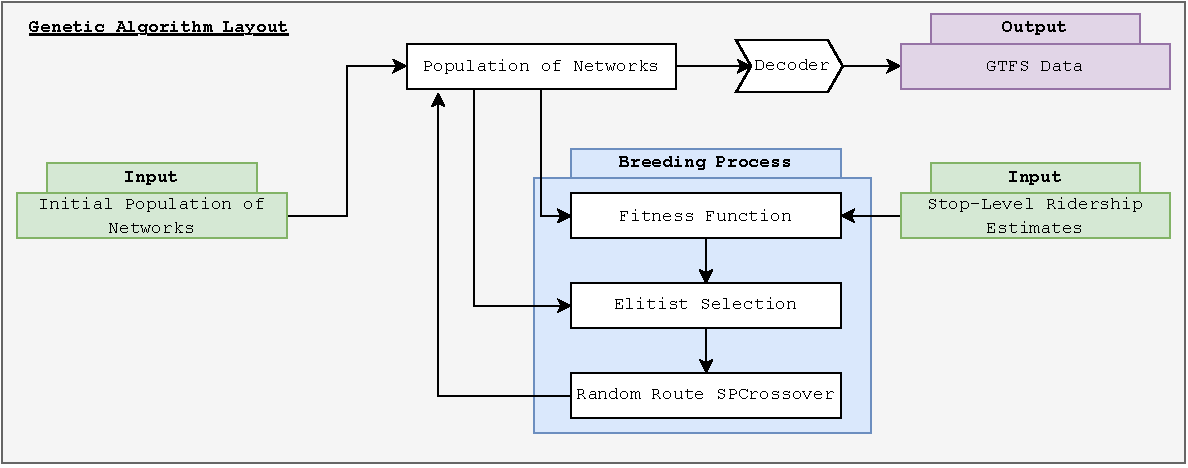
\includegraphics[width=\textwidth]{Thesis/diagrams/GeneticAlgorithmPlan.pdf}
    \caption{Transit GA}
    \label{diagram:my_ga}
\end{figure}

While many of the examples discussed in the introduction utilized a binary encoding of chromosomes, such an encoding is impractical in this application. Representing transit networks as a series of individual bits becomes increasingly complicated due to how we plan to work with the networks in our model. To highlight a few of these challenges, notice that networks may consist of different numbers of routes and routes themselves are likely of different length. While we could solve this issue via a ``messy'' GA approach where the encoding scheme is of variable length, this presents another challenge. Specifically, by representing the networks as some sequence of bits in a compact manner, the hierarchy of networks, routes, trips, and stops becomes difficult to maintain. Therefore, for the purposes of this algorithm, we choose to work directly with the networks rather than attempt to encode the representation directly into a string of bits. Specifically, the definition of a network within the implementation of the model allows us to maintain the natural hierarchy of the system from routes, to trips, and then to stops. 

Specifically, we wrap each member of the population in what we will refer to as a chromosome. Each chromosome has a network associated with it, as well as additional information for tracking purposes, such as the number of times it has been selected as a parent and a description of its 'family history': its parents, their parents, and so on until the initial population. 

 By working with this chromosome object, the logic of the computation becomes more natural. However, as a consequence, we must adapt crossover and mutation operations meant for binary strings to be applied to entire objects. 
 
 In the following sections, we more rigorously define what we mean by `improving' the transit system performance and how that will motivate our breeding process, and also how we define the core operations: selection and crossover. Both of which are tailored to the problem, and specifically the data, in consideration \cite{park2005}.
\subsection{Fitness Function}
Different fitness functions produce radically different results. Thus, this section describes the initial ideas behind a fitness function with the discussion in later sections taking on extensions or modifications of these original ideas. The initial fitness function for the algorithm is a very simple heuristic that assigns a value to each of the networks within the population. There are four main metrics we track to determine the fitness of some network $n$:
\begin{itemize}
    \item \textbf{Ridership($r(n)$):} In order to compute ridership, we sum the ridership over each stop of each route within a network. Specifically, we double count the stops that appear on multiple routes. This strategy rewards networks that include high-density or high-ridership stops in as many trips as possible. 
    \item \textbf{Coverage($c(n)$):} Coverage is approximated by looking at the number of distinct stops covered by the network in comparison with the original network. We then reward networks that span as many stops as possible, and punish those that exclude many stops. 
    \item \textbf{Complexity and Cost($u(n)$):} In this metric, we simply count the number of routes the network has, the idea being that servicing more routes requires more cost, and increases complexity, which in turn decreases usability and the frequency we are able to run each route. If a transit network has twice as many routes, each route can only be run half as frequently. Therefore, we want a low complexity to get low cost. 
    \item \textbf{Ridership Density($d(n)$):} This metric tracks the correlation between routes with a high number of transfers branching off of them and the ridership of each route. Ideally, we want these two numbers to be positively correlated since we want our routes with the most transfers to be the most popular. As an example, consider the opposite case: a route with very low ridership, but with transfers to everything. It is clear such a route serves little purpose in an effective transit system. 
\end{itemize}
In order to combine all of these metrics together into a single score for the network, we need to scale them to a similar scale. Therefore, all metrics are computed as a comparison with the original network created by $SFMTA$. For example, we define $R(n)$, the ridership score of a network as, 
\begin{align*}
R(n) = \frac{r(n)}{r(SFTMA)}.
\end{align*}
An analogous definition holds for $C(n)$, $U(n)$, and $D(n)$ as the scaled coverage, complexity, and ridership density scores respectively. This method of computing the metric also gives us an intuition for what the values represent where a value of 0.5 means half as good as the original, 1.0 means the same, and 2.0 means twice as good. 

We then take a weighted sum of these metrics to compute our fitness. If we define $N$ to be the space of all transit networks, then we can define $F: N \to \mathbb{R}^{+}$ as our fitness function on some network $n$ as follows:
\begin{align*}
    F(n) = \frac{(\lambda_{R} R(n) + \lambda_{C} C(n) + \lambda_{U} U(n) + \lambda_{D} D(n))}{(\lambda_{R} + \lambda_{C} + \lambda_{U} + \lambda_{D})}
\end{align*}
The hyper-parameters $\lambda_{m}$ for each metric $m$ denotes the weight placed on that metric in the overall fitness function. These weights serve as an opportunity for experimentation on the model's performance. 

Returning to the discussion of genetic algorithms, we want our model to be able to run with a large population size, and for many generations, in a reasonable amount of time, to reap the benefits of genetic algorithms \cite{mitchell1998}. Therefore, since the fitness function is going to be applied to each member of the population on each iteration, having a highly complex fitness function will significantly limit our ability to run the algorithm. Thus, the fitness function presented here is very simple and quick to compute. 

\subsection{Crossover Operation}
For our crossover operation, we present an intuitive idea based on single-point crossover whose details are ultimately a bit subtle. We call our crossover operation \textit{Stop-Point Crossover} (SPCrossover). Given two networks $N_A$ and $N_B$, we randomly select some pair of trips $(T_A, T_B)$ that meet the following criteria: 
\begin{itemize}
    \item $T_A$ belongs to $N_A$ and $T_B$ belongs to $N_B$. 
    \item $T_A$ is not the same trip as $T_B$. 
    \item $T_A$ and $T_B$ share at least one stop $S^*$ in which they approach in the same direction. 
\end{itemize}
Note that in order to determine if they approach the stop in the same direction, we use the direction attribute, a 0 or 1 to indicate inbound or outbound, associated with each trip in the GTFS data.\footnote{While some odd edge cases still exist in theory at intersections, such cases have not been found in experimentation.} Then, we perform single-point crossover on the lists of stops associated with each of $T_A$ and $T_B$ to generate two children trips from the resulting lists of stops. This is the same idea as expressed in Section 1.2.1 and demonstrated in Figure \ref{fig:singlePointCrossover}, with single bits  replaced by stops. For intuition, refer to Figures \ref{fig:crossover_1} and \ref{fig:crossover_2}.
\begin{figure}[h]
\centering
\begin{minipage}{.5\textwidth}
  \centering
  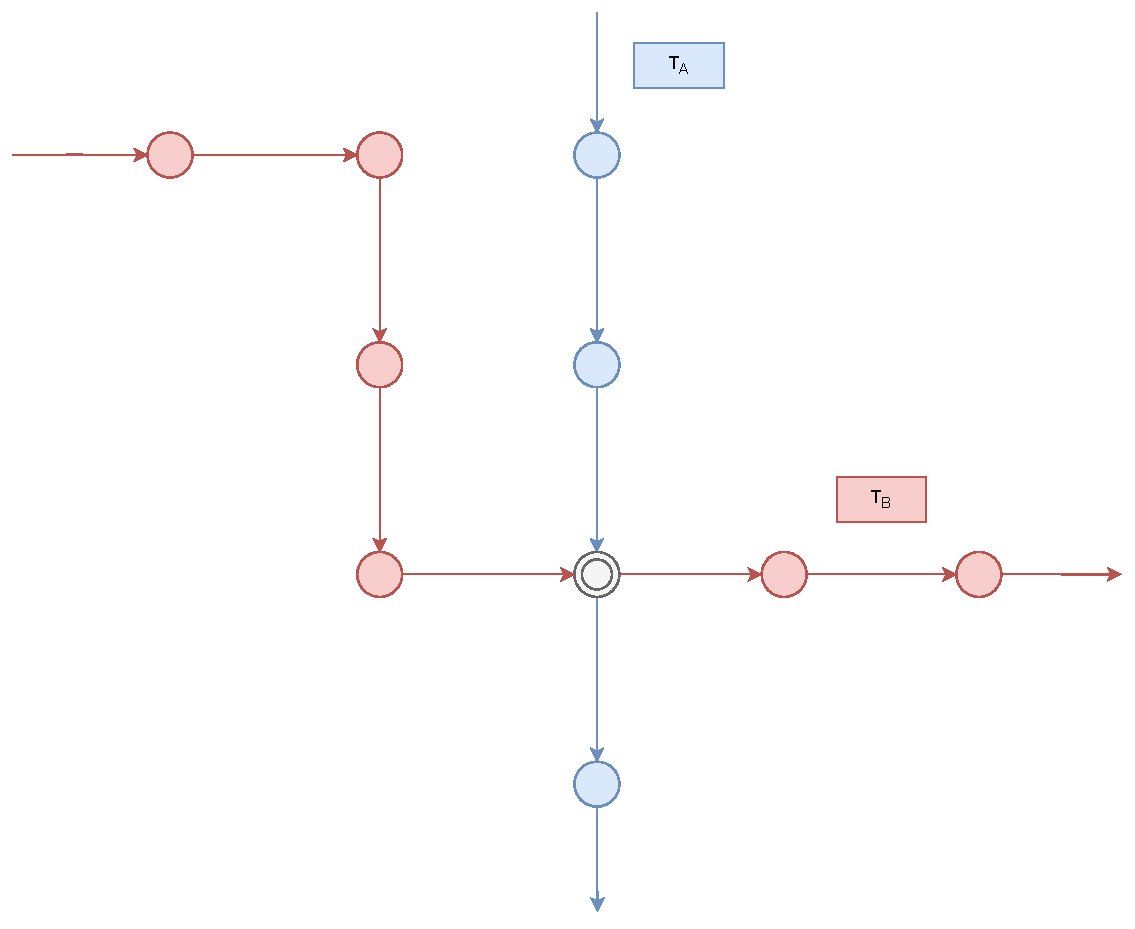
\includegraphics[width=\linewidth]{Thesis/diagrams/route-crossover1.pdf}
  \caption{Parent Routes}
  \label{fig:crossover_1}
\end{minipage}%
\begin{minipage}{.5\textwidth}
  \centering
  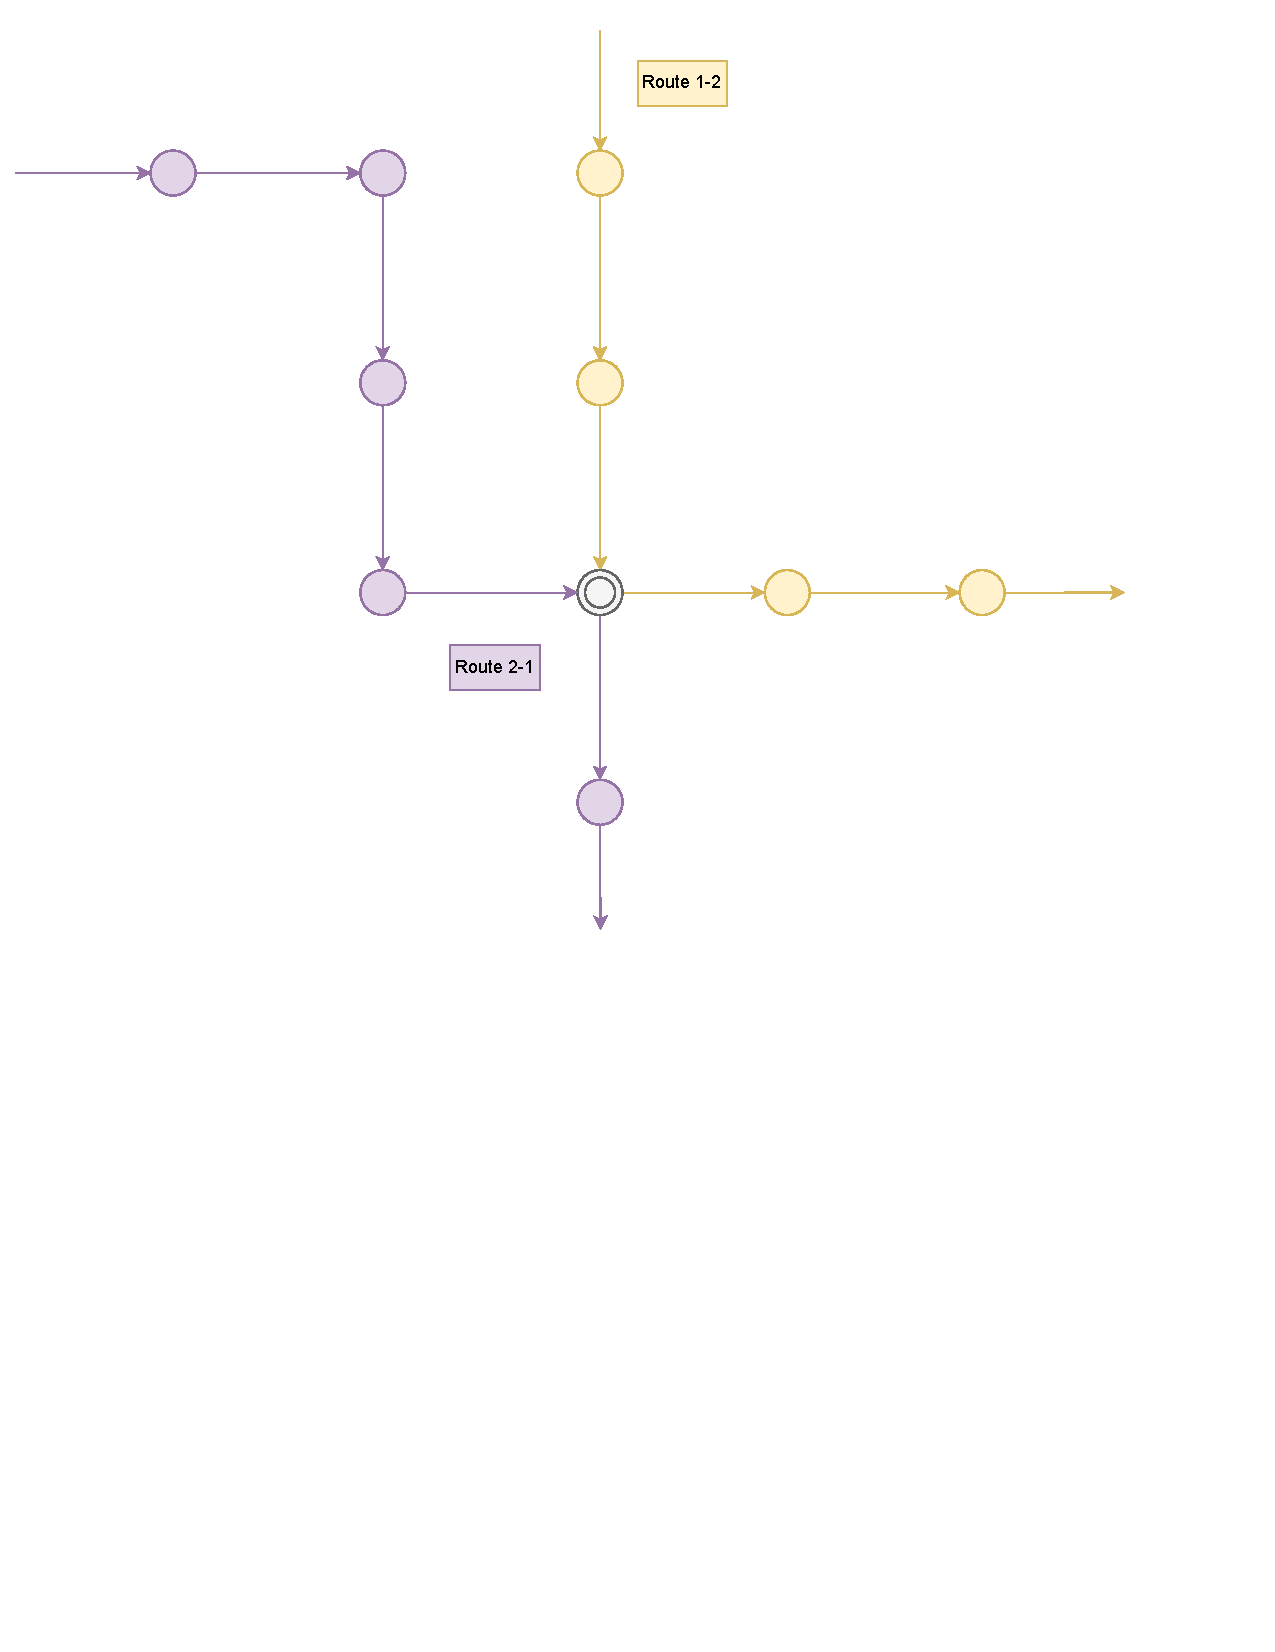
\includegraphics[width=\linewidth]{Thesis/diagrams/route-crossover2.pdf}
  \caption{Children Routes}
  \label{fig:crossover_2}
\end{minipage}
\end{figure}

Notice that this procedure describes how to form new child trips $T_{AB}$ and $T_{BA}$ from the parent trips $T_A$ and $T_B$ we selected. However, we still must produce networks from these trips. To do so, we copy one of the parent networks, either $N_A$ or $N_B$, at random, let the parent we choose be $N_p$. We initialize our new child network $N_c$ as a copy of $N_p$. Then, we add our new trips $T_{AB}$ and $T_{BA}$ to our new child $N_c$.  Finally, we remove $T_{A}$ and $T_{B}$ from our network $N_p$ if present. Notice that if either $T_{A}$ or $T_{B}$ are not in $N_r$, the parent we chose, the number of total trips of our child network $N_c$ could potentially be greater than its parents. 

Crafting the new child networks in this way allows us to keep the number of trips associated with any network from growing too rapidly. If we kept the parents trips along with their children in the new network, we would need an additional feature of the model to delete trips, otherwise the number of trips in our model would consistently grow since we would be adding two new trips to every child. However, such a deletion of trips would need to be at roughly the same frequency as they are being added via the breeding operation, otherwise the number of trips associated with each network would either grow without bound, or shrink down to zero. Because such a method for deleting trips is not part of this model, having the breeding operation keep this quantity from growing too quickly is vital. 

\subsection{Selection}
The final piece of the algorithm we want to address is how we select the parents $N_A$ and $N_B$ for SPCrossover and how we select a pair $(T_A, T_B)$. For selecting the parent networks $N_A$ and $N_B$, we implement an elitist selection where the top performing $E_{\text{cutoff}}$ fraction of networks from the previous generation live onto the next population. Then, within this subset of the population that lives on, we select potential parents randomly with weights according to their relative fitness. That is, if a network achieves a very high fitness score, it is very likely to be selected as a parent in the following generation. 

Secondly, in order to select a pair $(T_A, T_B)$ we rely on a randomized approach for more efficient results. We uniformly sample two trips, one from each network, and check if they meet the necessary criteria: intersect at some stop from the same direction and are distinct trips. Then, we use these trips, and this stop, as our pair. Note that if multiple stop intersections exist, we select a random one. However, if $(T_A, T_B)$ don't intersect at some stop, we sample new candidates $(T_A, T_B)$. We define $R_{max}=50$ to be the maximum number of retries to get an intersection. This conservative value was chosen since we observed that an intersection was almost always found within 10 tries.\footnote{If this does fail, which hasn't happened in practice, we return a copy of one of the parents at random as the new child. }

\section{Preprocessing: Working with GTFS and Ridership Data}

\subsection{GTFS Data}
In order to work with the GTFS and ridership data, significant work is needed before we can use it directly in our GA. Because of the format of the GTFS data, extracting the route data we are looking for requires a few steps. 

The GTFS data consists of a collection of files describing a hierarchy of objects within the transit system. It defines the following properties\footnote{These are only the pieces most relevant to this project. There is significantly more detail in GTFS detail that was omitted from this description.} of a transit system \cite{gtfs}: 
\begin{itemize}
    \item \textbf{Shape point:} a geospatial location specified by longitude and latitude coordinates. 
    \item \textbf{Shape object:} an ordered collection of shape points. A shape object describes a path in two-dimensional space. 
    \item \textbf{Stop:} a physical location where vehicles stop to unload and load passengers. Includes information about \textit{parent stations}. For example, a bus stop outside a larger train station would have the train station as a parent station.
    \item \textbf{Trip:} an ordered sequence of stops that occur in a specific direction at a specific time as well as a shape object describing how to get from one stop to the next. 
    \item \textbf{Route:} a collection of trips with similar or identical shape objects. For example, a route could be the two trips corresponding to the two directions of a bus carrying passengers from uptown to downtown and vice-versa. 
\end{itemize}

Notice that routes do not describe a direction or an ordering of stops, but rather only describe a collection of trips. It is at the trip level that the direction and ordering of stops is imposed. A route involve at least one trip going in each direction meaning that a route always describes at least two trips. However, in most cases it describes many other related trips that only stop at a subset of the same stops or run during different times of day. 

Additionally, the geometry of the route is stored with these shape objects which are linked to individual trips. Therefore, describing the shape of a route, or collection of trips, becomes difficult because it requires a way of combining the potentially different shapes within each trip. 

To simplify this problem, we will create what we will refer to as simple routes where we only consider the longest trip in each direction. Working with simple routes allows us to drastically reduce the number of trips to consider without losing any element of the geometry of the network.  

Moreover, we will define our simple routes to have simplified trips as well. Specifically, we want to ignore any stop that is not an endpoint of a trip or a transfer point. We define a transfer point as a stop that intersects another route of different shape. By specifying it this way, we avoid the case of two identically shaped routes utilizing the same stops, such as local and express lines.

More importantly, this simplification of the trips allows us to significantly reduce the number of stops we are working with and specifically focus on the geometry of how we connect transfer points and significant stops. This description of simple routes will appear more natural in the context of our crossover operation. 

However, note that the computation of such simple routes is not trivial. Specifically, we face two core challenges:
\begin{enumerate}
    \item \textbf{Determining transfer points}: identifying which stops are accessible via multiple routes. 
    \item \textbf{Assigning shape points to stops}: identifying which points of the shape objects of each trip are associated with each stop. 
\end{enumerate}

\subsection{Determining Transfer Points in GTFS} Unfortunately, stops are not marked as transfer points within the GTFS dataset. In order to determine such points, one could utilize the simple strategy of marking all of the stops used by each trip, then looking for stops that were marked by multiple trips. However, this will only catch trips that utilize the exact same stop, whereas it would fail to catch trips that utilize stops across the street from each other or just down the block. We use two methods to identify collections of stops that are close enough in distance to be considered transfer points. 

Since stops are described by longitude and latitude. We use Vincenty's formulae for calculating distance between points on a spheroid, as implemented in the \textit{geopy} package \cite{geopy}. 

First, we define some threshold $\delta_{stop}$ as the maximum distance two stops can be from one another and still be considered transfer points. Additionally, because the high level goal is to reduce complexity in the network, when multiple stops are within $\delta_{stop}$ of each other, we merge them into a single stop. This merging will reduce the number of stops significantly with very low impact on the overall geometry of the network, assuming a sufficiently small $\delta_{stop}$. Experimentation on real data was used to determine an appropriate threshold distance $\delta_{stop}$ of 100 meters.

Second, we can use the \textit{parent stop} field within the GTFS data. The parent stop field is part of a stop description and is often used to denote a hierarchy between the stops. Thus, rather than relying on a heuristic of threshold distance, in this case, we can identify transfer points by stops that share a common parent stop. Similar to above where we merged stops within a threshold distance, when we identify stops with a common parent stop, we will merge them into the parent stop. This again will reduce complexity in the network. 

In order to combine these two techniques, we first apply the parent stop method to merge stops into their parent stop. Then, we apply stop merging to further reduce the number of stops. Thus, by a combination of these two techniques, we are able to simplify the network further and identify transfer stops. 

\subsection{Assigning Shape Points}
Within SPCrossover as described in Section 2.4, the stops associated with each trip change. When a stop is added or removed, the shape of the trip itself could very likely change since it no longer visits the same stops. Therefore, we want to define the shape of a trip in such a way that it is function of which stops are included on the trip. That way, when we change the stops associated with a given trip, the shape of the trip can be updated. To define this function, we need to store the shape information of the trip within the stops included on the trip, rather than the trip itself. 

Suppose we have a trip $T$ with stops $s_1, \ldots, s_n$. A natural approach would be to compute the shape object that minimizes the sum of the distances between adjacent stops $s_i$ and $s_{i+1}$. However, computing such a shape is impractical in practice. First, the complexity of such a computation could become overwhelming when we consider a large transit network with many trips, each with many stops. Secondly, for these computations to be meaningful, significant data is required. Specifically, more data about the location of roads and their corresponding traffic laws would be needed, which would drastically increase the difficulty of the computation. 

Therefore, we simplify this calculation by assuming the existing route paths are already optimal, that is, the segment from any $s_i$ to $s_{i+1}$ is optimal in the existing transit network parsed from the GTFS data. Therefore, we can work with these segments when we want to add or remove stops from an existing trip. This then raises the problem of defining such segments which is where the idea of assigning shape points to stops comes into the picture. 

In order to assign shape points to stops, we need some way of knowing if a given shape point belongs to the segment between two given stops. Initially, to solve this problem, we make use of a simple heuristic that works as follows:
\begin{itemize}
    \item Let the current stop be the first stop on a trip. 
    \item Keep assigning shape points to the current stop until their distance with the stop begins to increase, suggesting we have passed the current stop on our route.  
    \item At that point, set the current stop to the next stop on the trip and continue. 
\end{itemize}
The intuition behind this idea is that we move along the shape of the trip, assigning the points to each stop until we pass it on our journey, where we then move on to the next stop. 

However, this algorithm was unable to account for more complex shaping in the routes. This becomes especially apparent when working with trips that turn around at some point, or move in shapes that turn back towards previous stops at any point. Therefore, a new heuristic is implemented. We make an assumption that there exists a shape point very close or essentially `on top of' each stop on a trip. The general approach is as follows:
\begin{itemize}
    \item For each stop associated with a given trip (in order of trip's direction): 
    \begin{itemize}
        \item Find the closest shape point in the shape object. Call it \textit{closest point}.
        \item Assign all shape points up to the \textit{closest point} in the shape object to the current stop. 
    \end{itemize}
\end{itemize}
This approach performed significantly better than the previous and was therefore chosen as the approach for partitioning shape points to stops within a trip. 

\subsection{Results in Network Simplification}
These heuristics show promising results in their ability to effectively simplify the network. To analyze this effort there are two key properties to examine in the simplified network: reducing network complexity while maintaining the shape of the network. 

\begin{figure}[h]
    \centering
    \begin{tabular}{|c|c|c|}
        \hline
         & Original GTFS Data & Simplified GTFS Data \\
         \hline
        \# of Routes & 128 & 53 \\
        \# of Trips & 49861 & 106 \\
        \# of Stops & 3282 & 546 \\
        \hline
    \end{tabular}
    \caption{Statistics on Network Simplification}
    \label{table:num_changes}
\end{figure}

To investigate the results concerning the first property, Figure \ref{table:num_changes} shows us that the complexity is significantly reduced. Specifically, notice the number of trips drops drastically since we only consider the longest trips associated with each route and do not worry about trips at different times, days of the week, or modified trips. Also notice that the number of routes was reduced significantly by only considering routes with active ridership. The GTFS data contains data on routes that may no longer be active or receive significant ridership. A common explanation being that many routes are temporarily suspended due the pandemic and plan to reopen to riders soon. 

\begin{figure}[h]
\centering
\begin{minipage}{.5\textwidth}
  \centering
  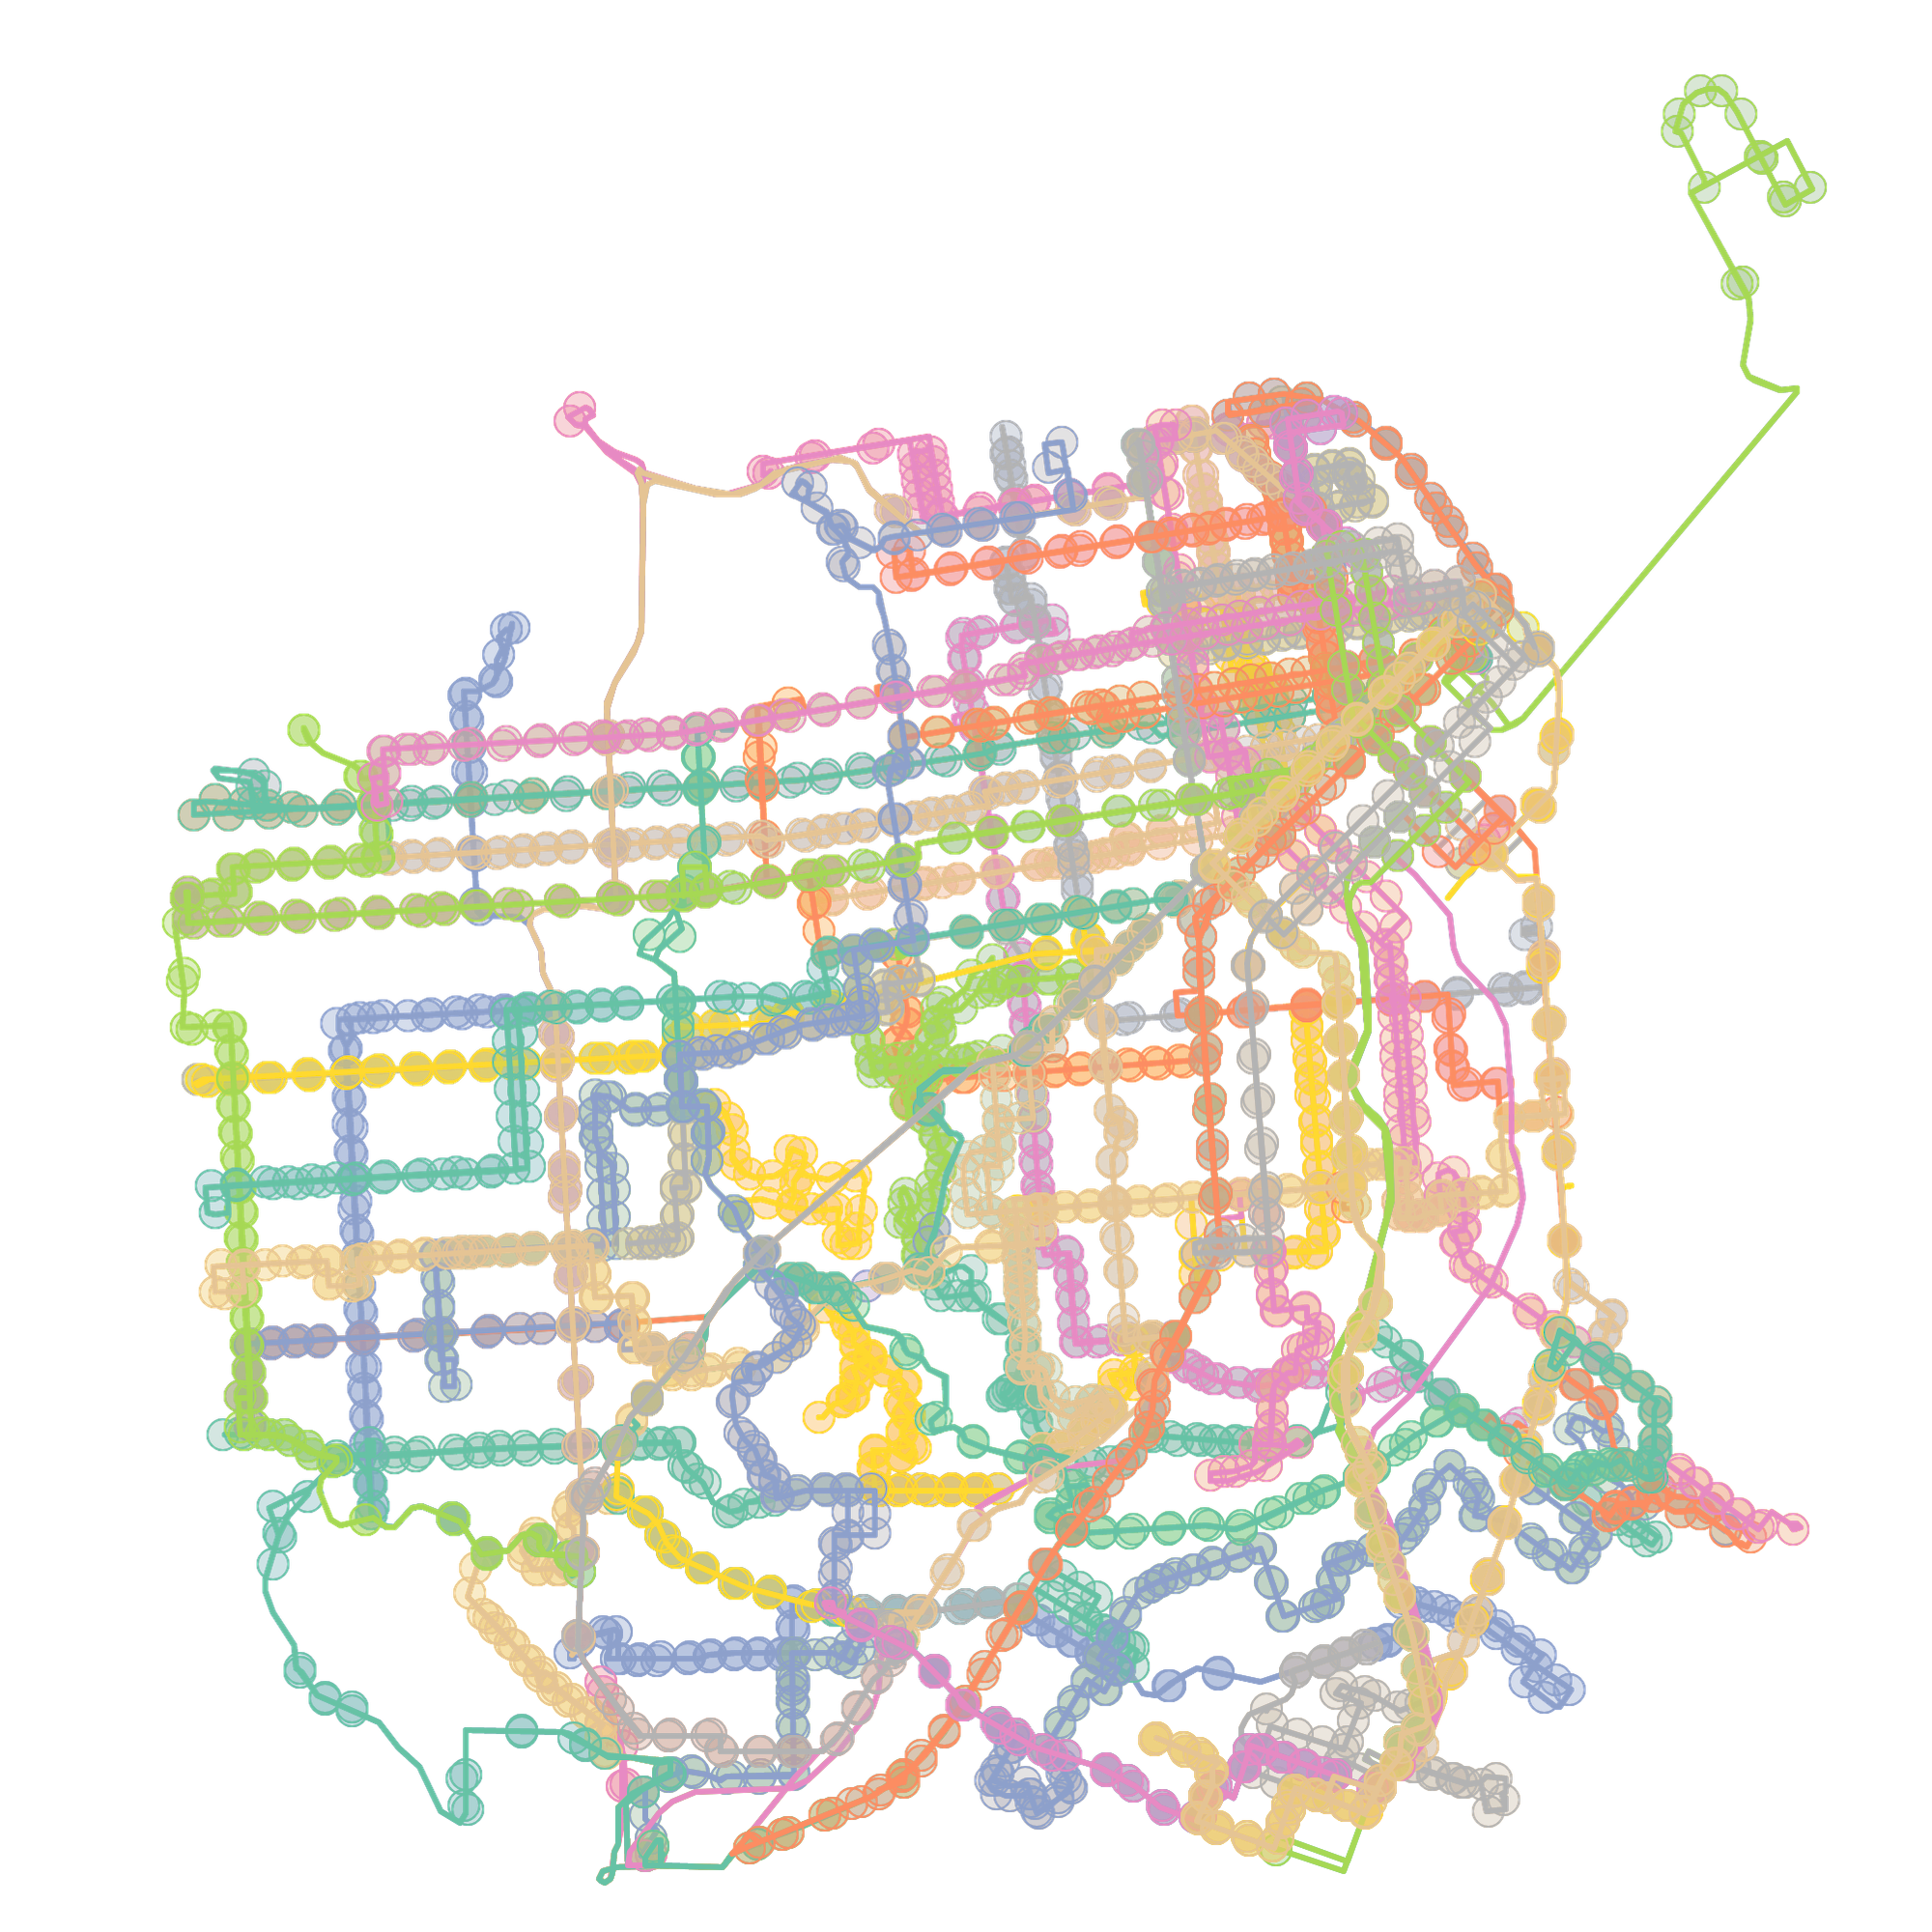
\includegraphics[width=\linewidth]{Thesis/diagrams/original_network.png}
  \caption{Original Network}
  \label{fig:original_network}
\end{minipage}%
\begin{minipage}{.5\textwidth}
  \centering
  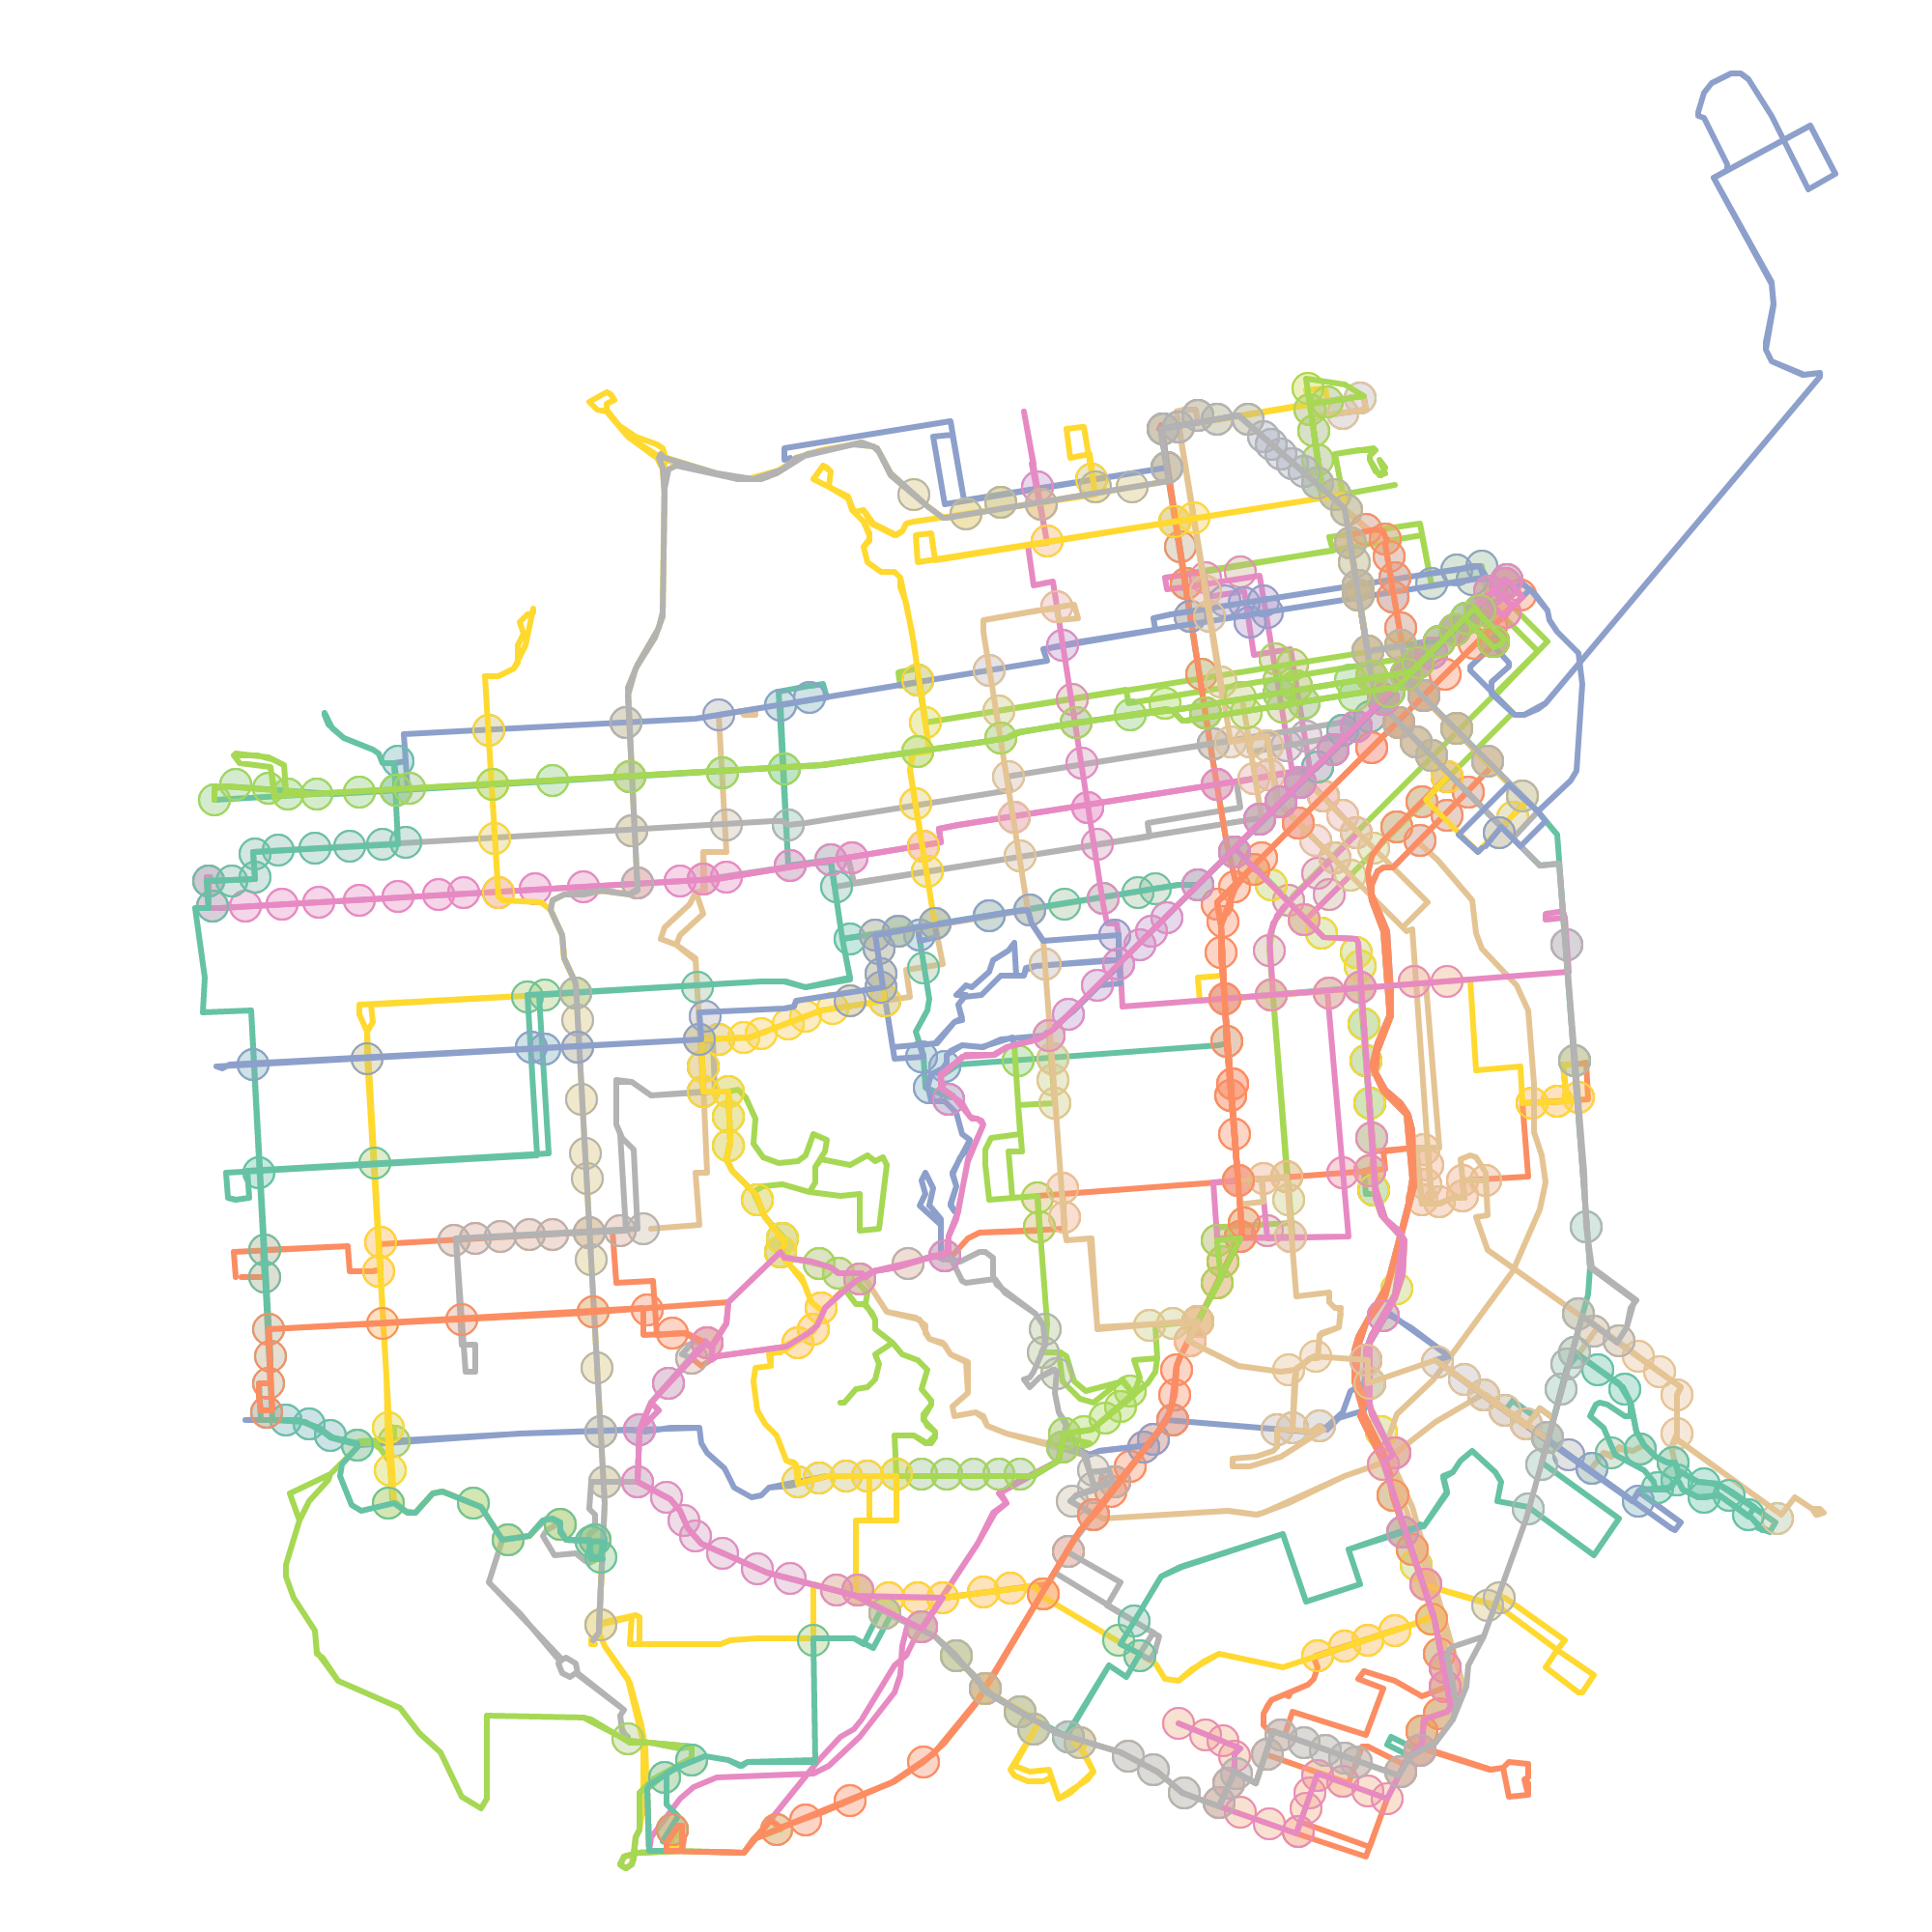
\includegraphics[width=\linewidth]{Thesis/diagrams/simplified_network.png}
  \caption{Simplified Network}
  \label{fig:simplified_network}
\end{minipage}
\end{figure}


The second question is much easier to consider visually. Figures \ref{fig:original_network} and \ref{fig:simplified_network} compare the two networks.\footnote{The difference in color is a result of the graphing used and does not reflect additional information.} In these figures, the colored lines represent the shape of the route and the dots along the way represent stops. That is, the colored lines are the shapes the bus make when they traverse a trip and the dots are where they stop to pick up or drop off passengers. By comparing these figures it becomes increasingly apparent the reduction in complexity of the network. Additionally, one can see that the shape of the network is completely unchanged, indicating that we are successful in simplifying the network without compromising on working with the true geometry of the network. 

\subsection{Ridership Data}
The data provided for ridership involves route level estimations by month performed by SFTMA officials \cite{SFMTA}. However, in order to work with this data more effectively in the context of this project, we need stop-level estimations. Therefore, we develop a method of estimating stop level ridership from route level values. Notice that this involves the challenge of appropriately assigning ridership to each trip within a route, and then from there to each stop. 

This subproblem of estimating stop level ridership from other data and factors is its own complex and well studied problem. Specifically, it has been shown that the two most important factors influencing boarding at the stop level are the urban density of the stop location and frequency of transit routes in the surrounding area \cite{baek2016, gutierrez2011}. Because we are only working with transit data, we will use transfer points exclusively to identify stops of higher ridership. 

For each stop, we will add ridership independently for each route stopping at that stop. Therefore, stops with more transfers will be rewarded with much higher ridership.  

For a single route $R$ with ridership $Rd$ and stops $s_1, \ldots, s_n$, we increment the ridership associated with each stop $s_i$ by $\frac{Rd}{n}$. Doing this for each route in the network results in significantly higher ridership associated with transfer points since they are counted for each route that intersects them. This idea is in line with the work done in stop level estimation outlined above and it simplifies the data processing involved in this model.

\subsection{Generating Initial Network Population}
In order to form an initial population, we make use of the SFMTA network design. Since our encoding scheme consists of working with objects directly, we do not have the luxury of generating random encodings, knowing they correlate to some possible network. Thus, instead, we breed a new population up from the original. Specifically, we take two copies of our initial network, the SFMTA network, and breed them to get a third. Then, with a population of three, we uniformly sample from the population to select parents to breed the next one. We repeat this process until reaching the desired population size. 

This approach poses strong advantages and disadvantages. First, as an advantage, it is efficient and easily computable. All the functionality needed is already built into the model itself. If we consider the alternative of attempting to generate random networks from scratch, we must answer questions about feasible routes, the legal paths they can take, and where good stops could be placed. Such questions are out of the scope of this project as they require significant GIS data analysis. 

This method has the disadvantage of an inherent lack of diversity within the initial population. Since all networks are bred from the initial starting network, the genetic diversity is very low. This concept of genetic diversity is critical to the success of genetic algorithms \cite{holland1992}. A larger genetic diversity, particularly at the initial stages, results in a larger search space for potential solutions and thus better performance. Unfortunately, genetic diversity can only be measured indirectly by the performance and attributes of the chromosomes within the population. 

 In order to estimate this quantity, we can look at the physical attributes, such as number of routes, of the network as well as its fitness. See Figure \ref{table:initial_pop_data} for an example of such statistics. 

\begin{figure}[h]
    \centering
    \begin{tabular}{|c|c|c|c|c|}
        \hline
        Metric & Mean & Median & Standard Deviation \\
         \hline
        Ratio of \# of Routes to SFMTA & 0.947 & 0.946 & 0.019 \\
        Ratio of \# of Trip to SFMTA & 0.947 & 0.943 & 0.018 \\
        Ratio of \# of Stops to SFMTA & 0.999 & 1.0 & 0.001 \\
        Ratio of Fitness Score to SFMTA & 0.924 & 0.926 & 0.031 \\
        \hline
    \end{tabular}
    \caption{Statistics on Initial Population (N=1000)}
    \label{table:initial_pop_data}
\end{figure}

Experimenting with other methods of initial population generation seems needed as the genetic similarity in the initial population is clearly very low in the current approach. 


\subsection{Summary of Preprocessing}
To summarize the work done in this step, refer to Figure \ref{diagram:Preprocessing}.\footnote{Note that the encoding scheme refers to representing the transit networks as the objects themselves, and not a traditional binary encoding.}
\begin{figure}[h]
    \centering
    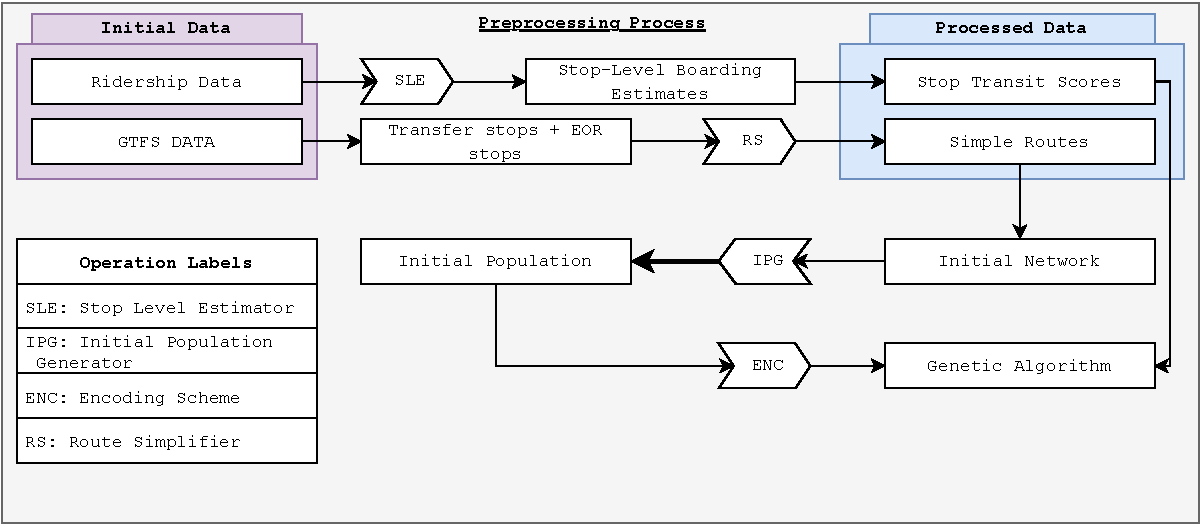
\includegraphics[width=\textwidth]{Thesis/diagrams/preprocessing_steps.pdf}
    \caption{Preprocessing Flow Chart}
    \label{diagram:Preprocessing}
\end{figure}

\section{Initial Results}

\subsection{Hyper-parameters Worth Exploring}
Because of the complexity of the algorithm, there are many potential areas for exploration in terms of how different hyper-parameters affect the types of the network the genetic algorithm rewards and produces in later generations. Two key hyper-parameters are \textit{population size} and \textit{maximum generation}. Population size determines how many chromosomes, or networks, to maintain in our population. Maximum generation determines the number of rounds to run the model before terminating. As previously discussed, high genetic diversity is important for the success of genetic algorithms. Therefore, the higher the population size, the better. However, a larger population is slower to run individual generations, meaning less time for experimenting with other hyper-parameters. 

Similarly, the maximum generation number is correlated with time and computational power. In contrast to population size, there are diminishing returns to increasing the number of iterations. Generally, the initial population of a genetic algorithm is the most diverse of the bunch, and slowly, the entire population converges to a less genetically diverse population. Therefore, running more iterations of the algorithm once it has already converged to a certain degree, is not nearly as fruitful as the initial iterations. 

Therefore, in order to determine an effective number of iterations, we keep detailed metrics on the distribution of the population characteristics, and particularly the standard deviation among the characteristics such as fitness and the factors that contribute to it in order to estimate the genetic diversity of our population. 

\subsection{Initial Fitness Function Performance}
For the purposes of this section, we will arbitrarily fix $N=1000$ as our population size and $l = 100$ as our number of generations. Initially, the coefficients are set as depicted in Table \ref{table:coefficients_1}.\foottnote{While these weights do allow for negative fitness scores for large enough $U$, such fitness scores were not observed in practice. Additionally, all fitness scores are taken to be the maximum of $0$ and result of $F(n)$ to avoid issues with parent selection.} These coefficients determine the weight each factor holds in the overall fitness function. The statistics regarding fitness per round is depicted in Figure \ref{fig:first_run_fitness}.

\begin{figure}[h]
    \centering
    \begin{tabular}{|c|c|}
        \hline
        Parameter & Value \\
         \hline
        $\lambda_{R}$ & 1\\
        $\lambda_{C}$ & 1\\
        $\lambda_{U}$ & -1\\
        $\lambda_{D}$ & 1\\
        \hline
    \end{tabular}
    \caption{Values of hyper-parameters}
    \label{table:coefficients_1}
\end{figure}

\begin{figure}[h]
    \centering
    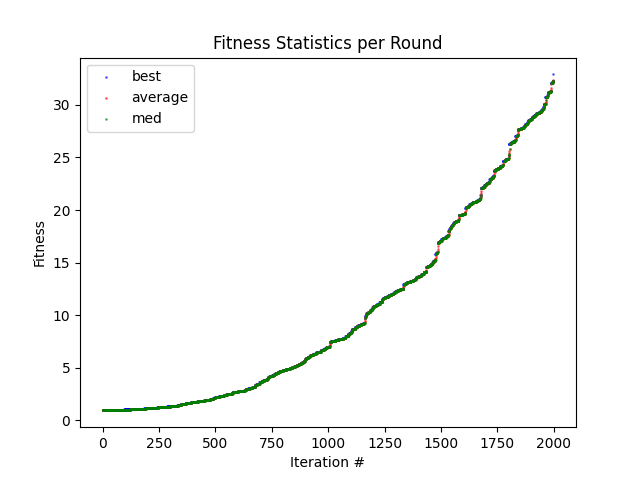
\includegraphics[width=\textwidth]{Thesis/diagrams/first_run/fitness_trend.png}
    \caption{Fitness by Round}
    \label{fig:first_run_fitness}
\end{figure}

Recall that the scale for the fitness assessment is with respect to the fitness of the original network. That is, 1.0 score of fitness corresponds to equal fitness to the SFMTA network and a 2.0 corresponds to double the fitness. With these hyper-parameters, we notice that the fitness starts off with slow growth, then accelerates into a fast constant growth. A trend worth noting is that the best fitness can make large leaps in between generations, whereas the average and median are slow to catch up. When we have some chromosome that performs very well in a given generation, its probability of becoming a parent for new networks in the next generation is very high. Thus, it will propagate its genetic material into the population, causing an overall increase in fitness. 

We can also look at how each factor of our current fitness function contributes to our overall fitness in Figure \ref{fig:first_run_fitness_breakdown}.\footnote{Note that the values for coverage and ridership are on top of each other in the figure, making it difficult to distinguish them.}

\begin{figure}[h]
    \centering
    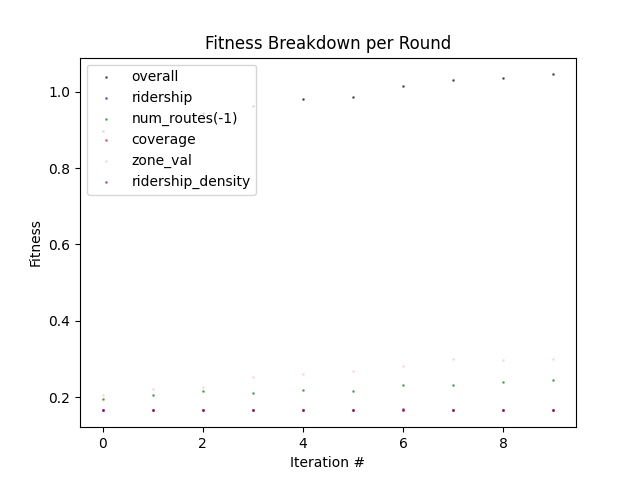
\includegraphics[width=\textwidth]{Thesis/diagrams/first_run/fitness_breakdown.png}
    \caption{Average fitness breakdown by round}
    \label{fig:first_run_fitness_breakdown}
\end{figure}

It is immediately apparent that the ridership density is the explanation of the rapid explosion of fitness values. Recall that ridership density rewards networks with many high-ridership routes that also have a high number of transfers. However, some of the other factors seem less influential. First, coverage as well as ridership remain constant. Coverage is measured as the number of total stops within the network, and when breeding a network, it is not possible to add more stops to the network, only change which routes go through them. Thus, the amount of fitness contributed by the coverage cannot grow making it a poor parameter for our fitness function. While it is possible for coverage to drop through our breeding operation, that doesn't appear to be happening in the population suggesting that the breeding operation is preserving the total number of stops or that any drop in stops causes a network to not live on to the next generation.  

Additionally, raw-ridership count also appears to preserved by the breeding operation and therefore also makes for an uninteresting metric to include in our fitness function. The final metric we include in our fitness function is the number of routes within the network. The number of routes appears to grow roughly linearly with the iteration number suggesting that network complexity inherently increases as the algorithm continues. The more generations in, the more likely a network is to have more new routes from breeding. Thus, it becomes clear why this value appears to grow in a linear fashion. 

Another aspect of the model worth highlighting is the standard deviation of different metrics as a means of estimating genetic diversity as seen in Figure \ref{fig:first_run_stddev}. 
\begin{figure}[h]
    \centering
    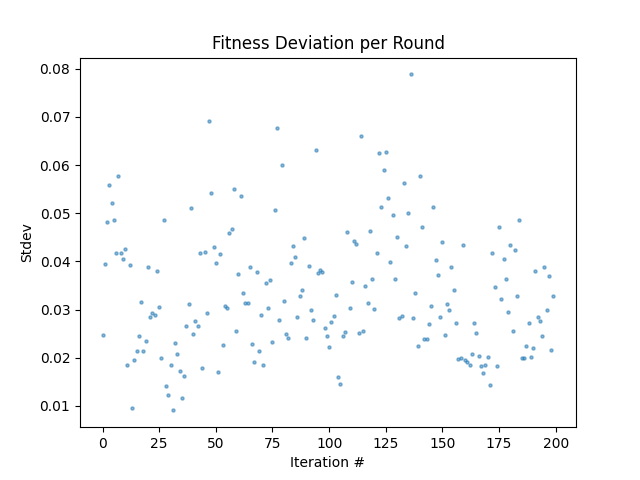
\includegraphics[width=\textwidth]{Thesis/diagrams/first_run/stddev.png}
    \caption{Deviation of fitness by round}
    \label{fig:first_run_stddev}
\end{figure}
The deviation increasing each round at an accelerating rate is unexpected and signals a flaw within the model. Returning to the view of genetic algorithms as a search technique, an increasing genetic diversity implies that the search is not converging, but rather diverging. 

One possible cause could be the lack of initial genetic diversity in the population. Recall that the high-level goal of a genetic algorithm is to randomly explore a search space with heuristics to attempt to find a local maximum at which it will converge. However, if the population begins very concentrated in that search space, and is not at a local maximum, the algorithm will continue to reach out randomly until it finds a point of convergence. This idea could be used to explain the increasing genetic diversity within the population of networks. That is, the initial networks are all very similar, but are not optimal. Therefore, the algorithm is rewarded by creating network more and more different from each other, resulting in higher genetic diversity. A product of this explanation is that the SFMTA network does very poorly with respect to this fitness function compared to other networks. The further the networks get from the original, the more they are rewarded, and therefore the worse the starting point appears. This relationship deserves more thorough investigation with other fitness functions and other hyper-parameters to see if this is due to a biased fitness function rewarding poor-transit design, or if this is exposing design flaws within the SFMTA design.

If this theory holds, we would expect that at some point the genetic diversity stops growing and begins to decrease. In order to test this, we can run the algorithm for more generations and specifically track how the standard deviation fluctuates round to round. If the population is observed to continue increasing its fitness, this likely highlights a flaw in the fitness function design in that it doesn't describe a problem with a defined optimal solution, but rather is unbounded. In the following section, we analyze the top performing network from the final generation and explain how it illustrates flaws in the fitness function. 

\subsection{Examining Resulting Networks}

The networks produced by the current fitness function clearly illustrate a flaw in the initial design. Specifically, with all fitness metrics, we reward longer trips that span the entire city. For example, in the case of ridership density, if the network can have a \textit{super-route} covering most of the city, and thus have transfers and high estimated ridership, the ridership density score will be very high. Refer to Figure \ref{fig:first_run:best_performer} for a graph of the best performing network in the final generation, as well as Figure \ref{fig:firt_run:long_route} as an example of one of its \textit{super-routes}. Note that many of its routes were ultimately very long, with few total routes. 

\begin{figure}[h]
\centering
\begin{minipage}{.5\textwidth}
  \centering
  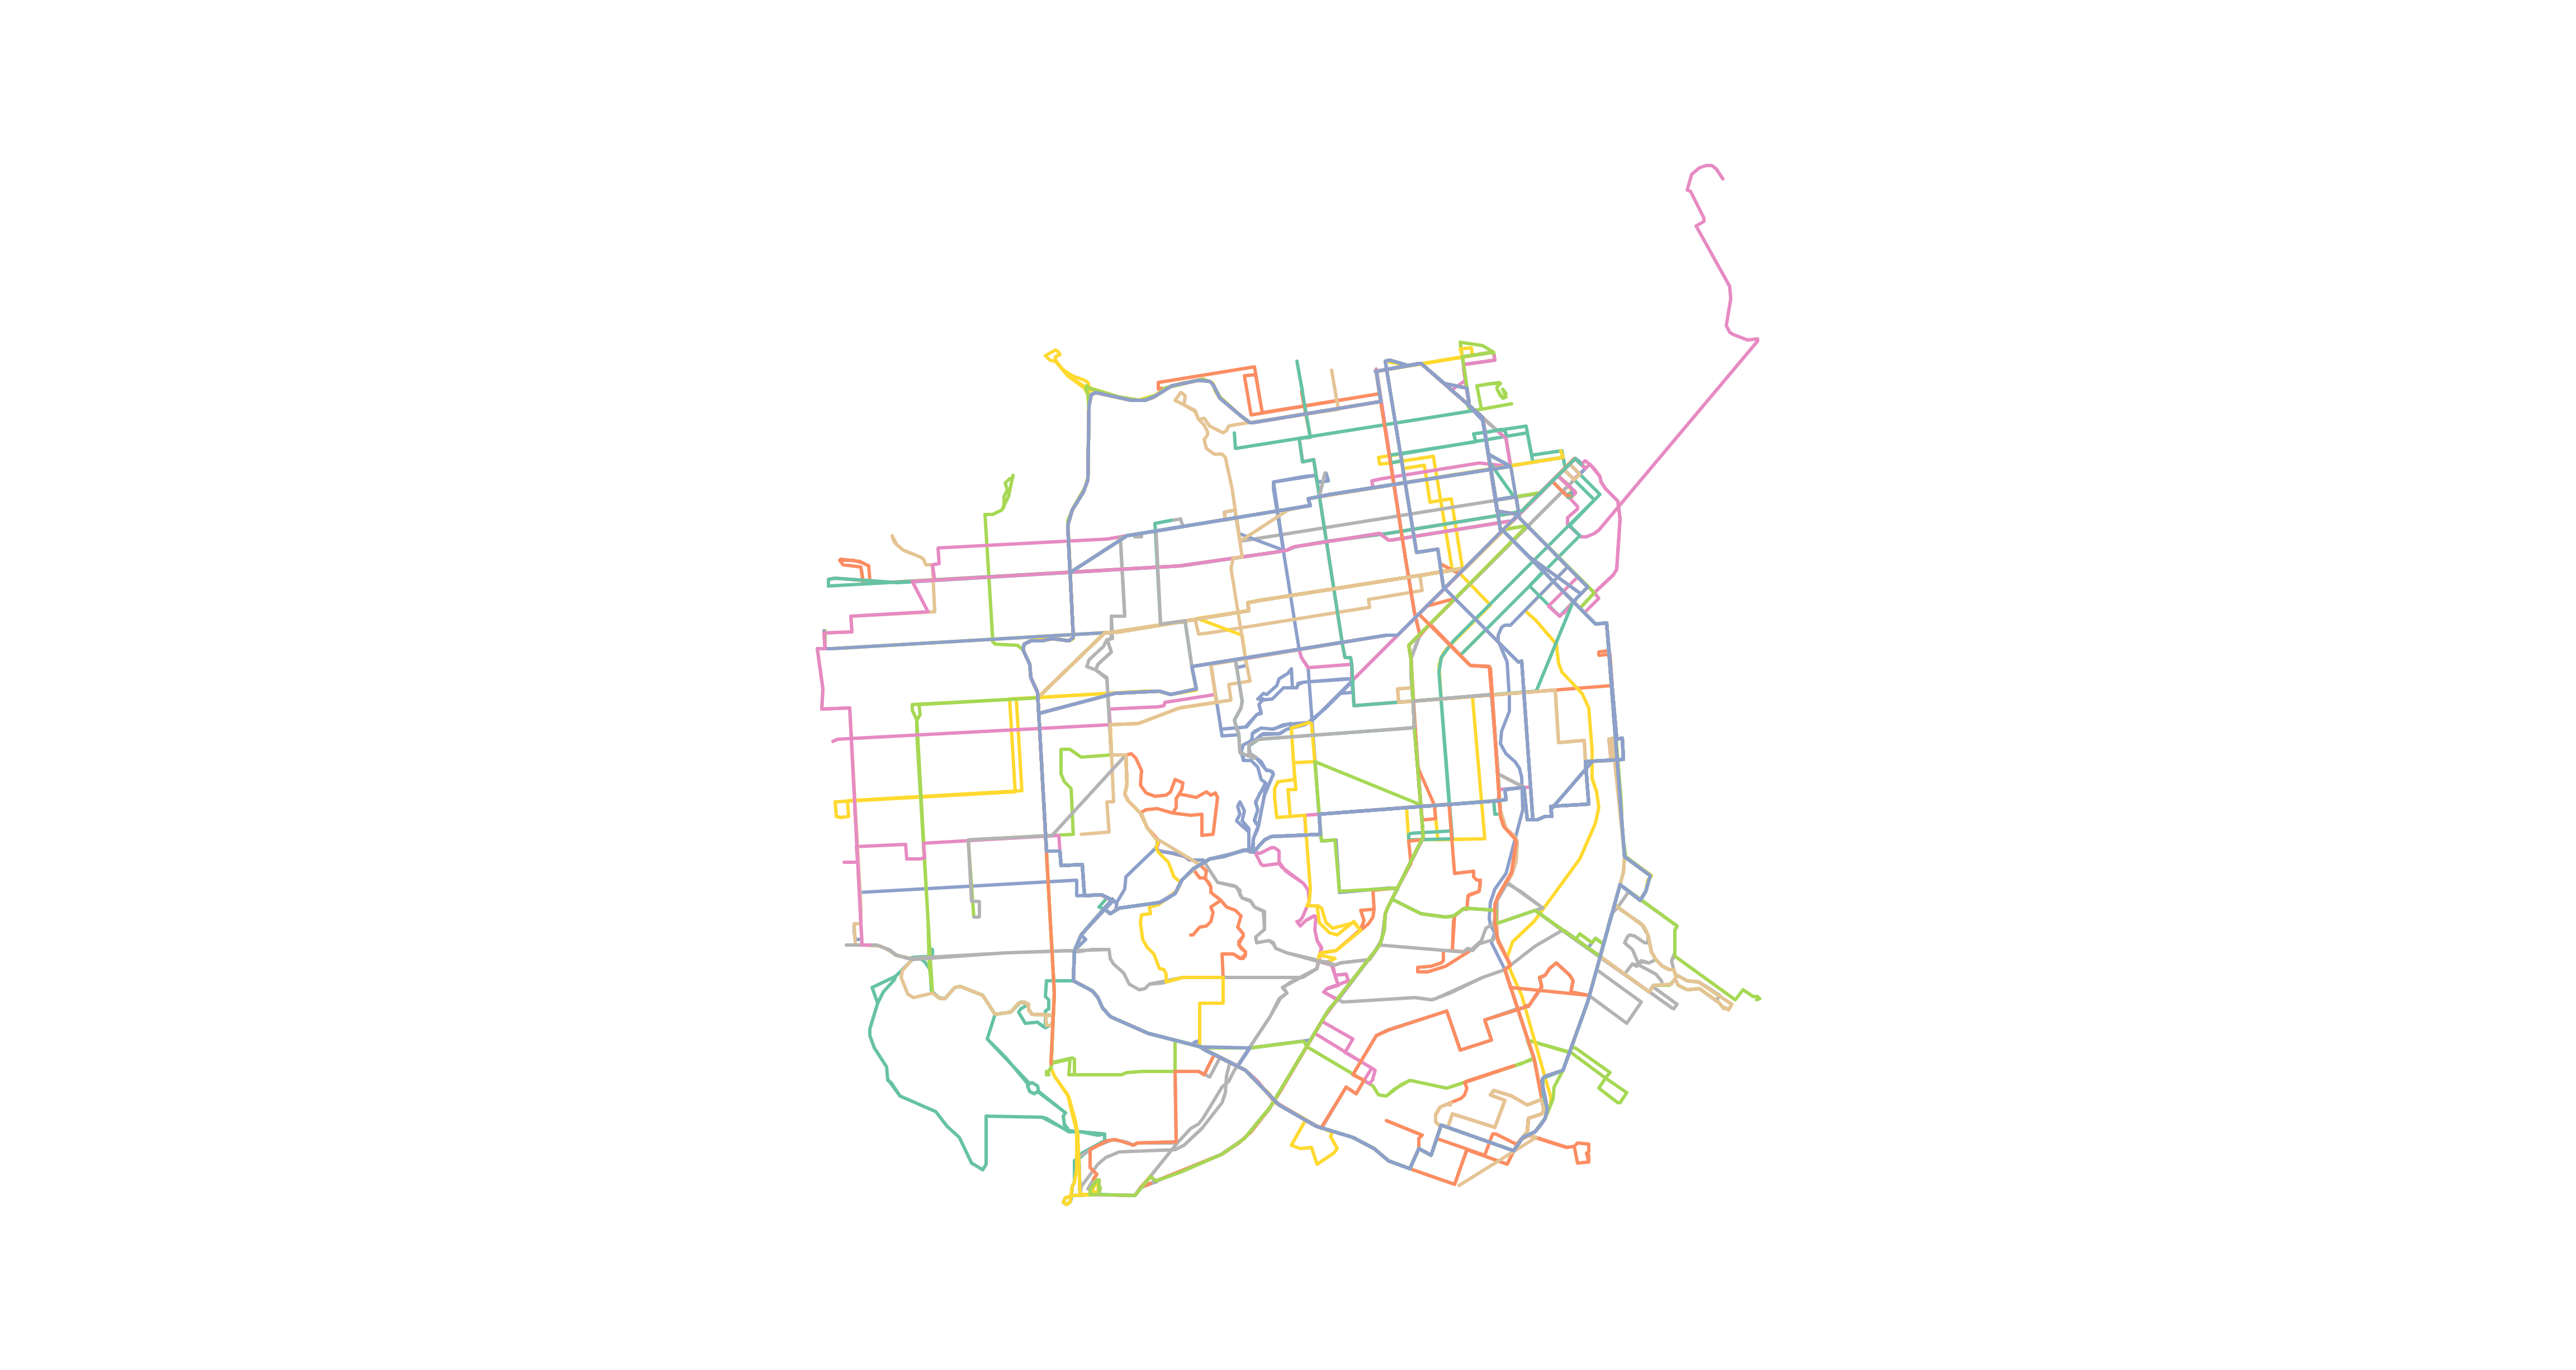
\includegraphics[width=\linewidth]{Thesis/diagrams/first_run/best_performer.png}
  \caption{Highest fitness in final generation}
  \label{fig:first_run:best_performer}
\end{minipage}%
\begin{minipage}{.5\textwidth}
  \centering
  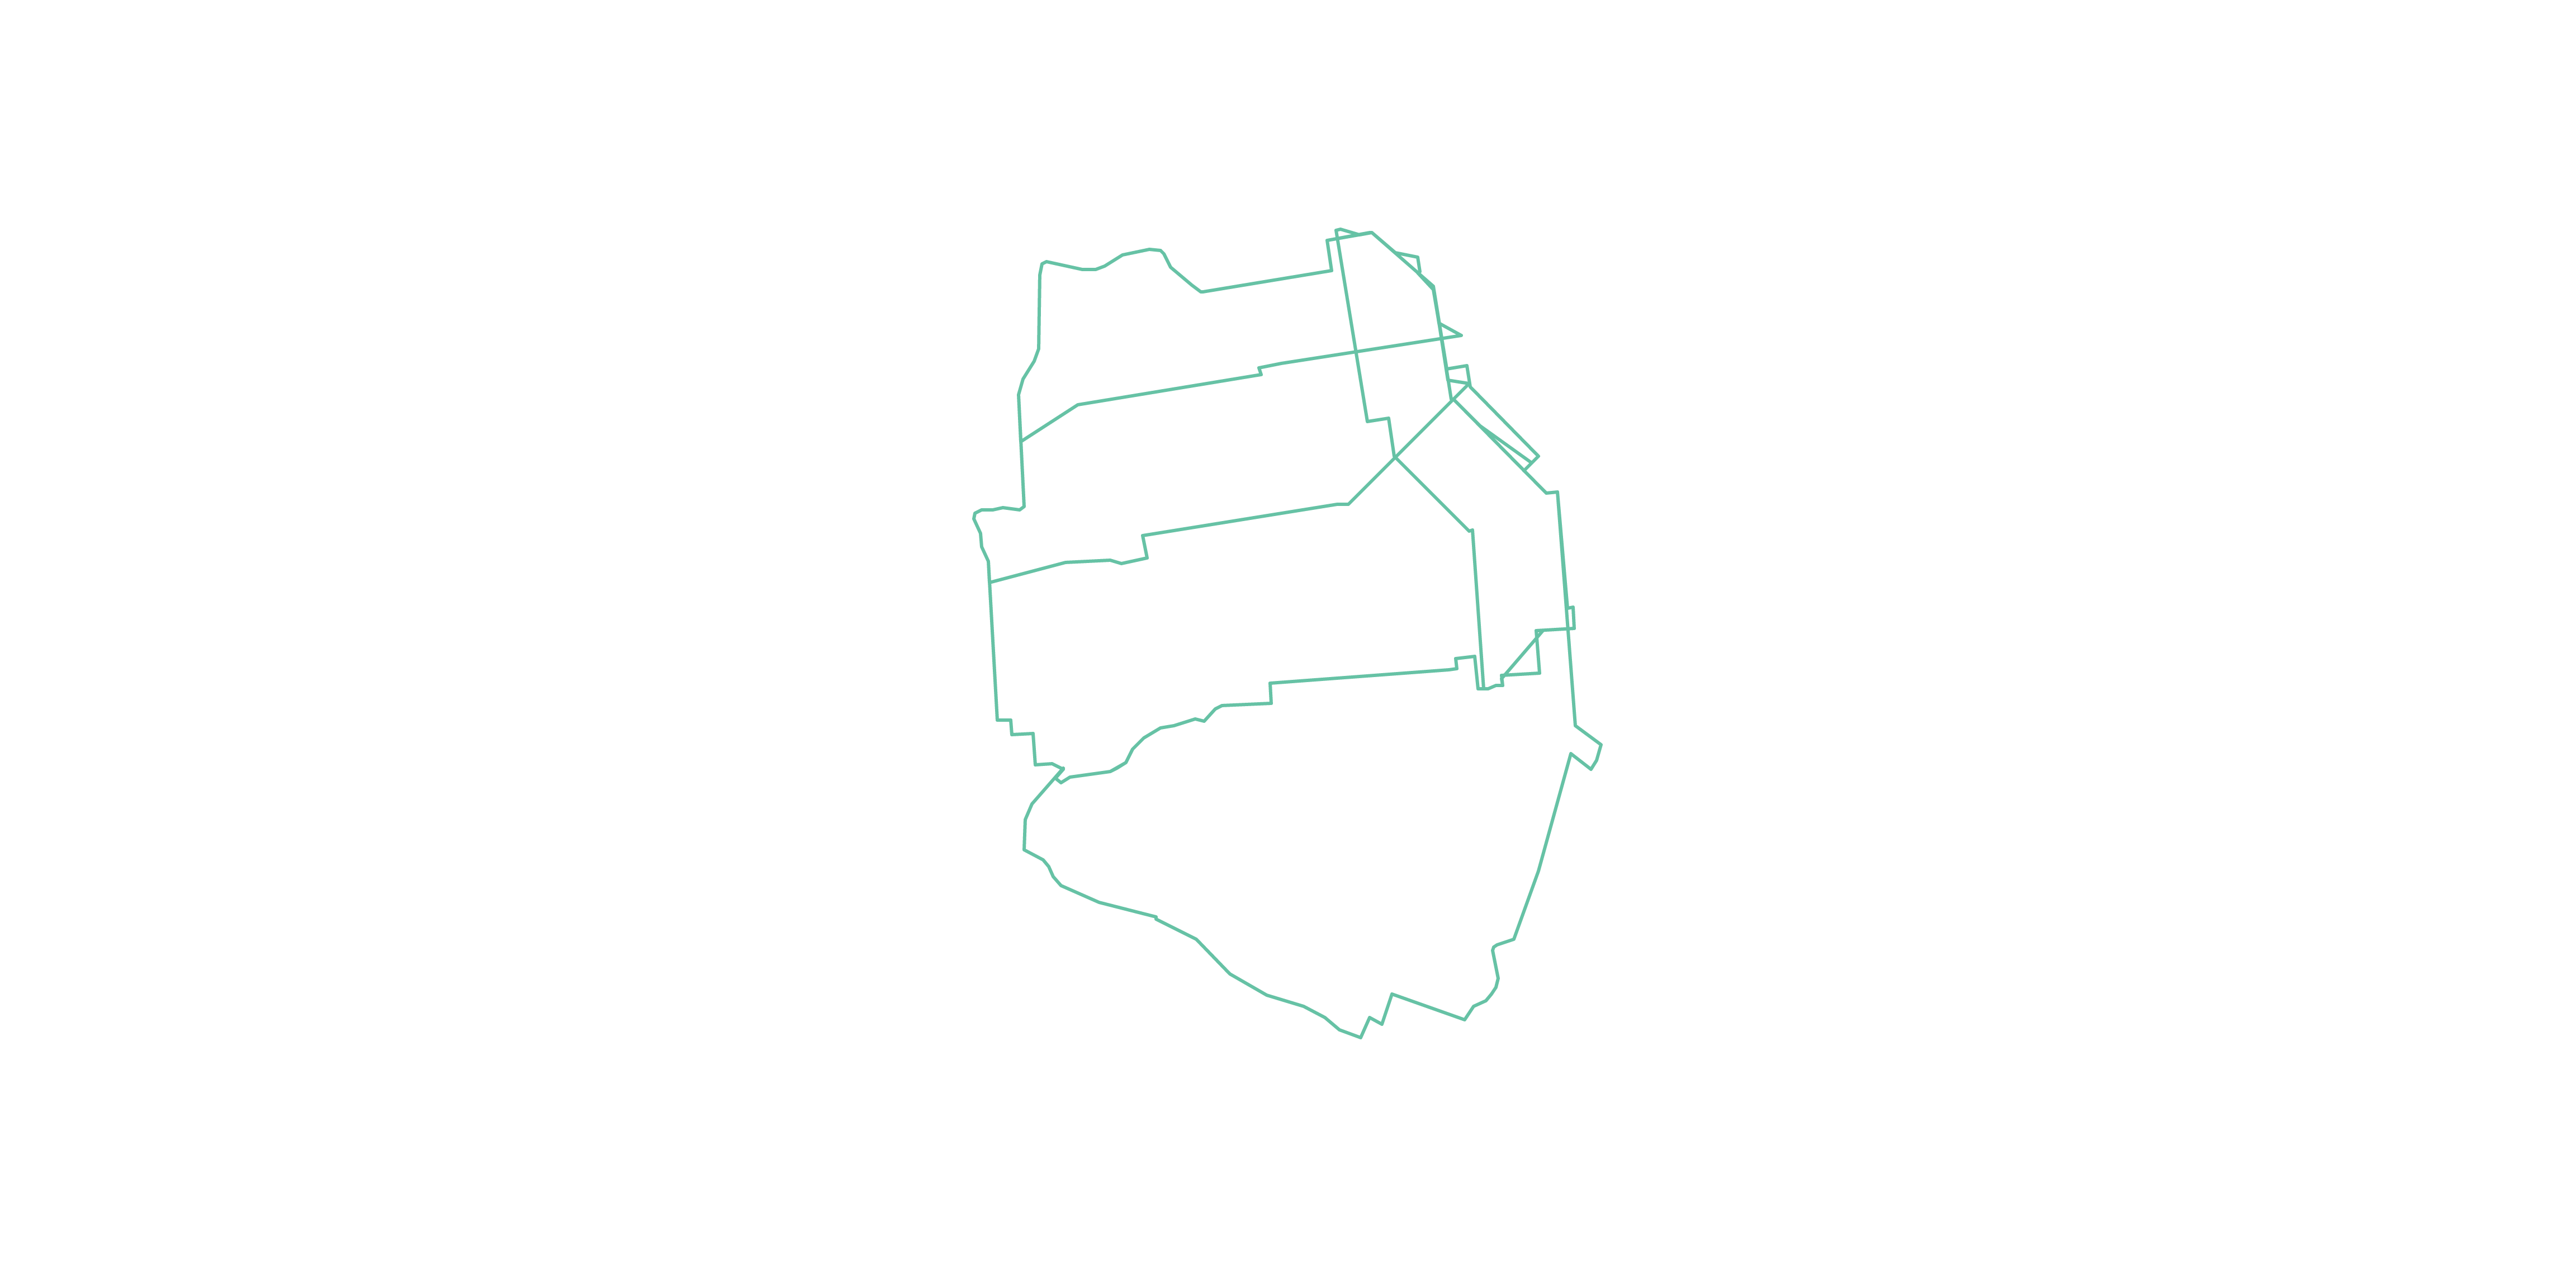
\includegraphics[width=\linewidth]{Thesis/diagrams/first_run/long_route.png}
  \caption{A long route on the new network.}
  \label{fig:firt_run:long_route}
\end{minipage}
\end{figure}
However, in reality such routes are impractical due to the inherent inefficiency for passenger use. That is, a passenger trying to go from one place to another is forced to stop at many locations irrelevant to them before getting there, and is forced to a take a tour of the city before arriving at their destination. Thus, the efficiency of the routes and their ability to bring people from one location to another in a timely manner must be incorporated into the fitness function. 

Despite these initial results producing an unrealistic transit network, they highlight the power of genetic algorithms. Given a fitness function, the genetic algorithm excels at finding ways to maximize the function in any way possible given its structure, even if that means forming super-routes that span the entire city. 

Returning to the theory from the previous section of lacking initial genetic variation, this flaw in the fitness function suggests that a mix of two options outlined was correct. That is, the initial network population is not optimal and therefore the algorithm diverges from it aggressively, increasing the genetic diversity throughout the generations. However, the reason it is not optimal is due to a flaw in the fitness function rewarding the creation of super-routes that span the city. In addition, it still could be true even without the creation of these super-routes, we get a diverging population due to an initial lack of genetic diversity. 

\section{Model Improvements} 
To improve on the initial version of the model, we add a few extensions and tweaks, whose details are described in the following sections. These changes aim to address the shortcomings seen in the initial results as well as enhance the model's ability to produce realistic and effective networks. Directly from the initial results, we remove the ridership and coverage metrics from the fitness function since they did not appear to vary in the population. In their place, we add two new fitness metrics. 

First, we want to address the super-route issue from the initial runs of the model. Since these routes are not practical in a real world setting, we add a constraint of realistic route length. Specifically, by examining the distribution of route lengths that SFMTA is currently running, we set a range of acceptable trip lengths, and punish networks that include many trips outside of that range. 

Formally, we define $e(n)$ to be the \textit{extreme trip score} of a given network $n$. We have lower and upper bounds $L_e$ and $U_e$ for the acceptable trip lengths. Then, for each trip $t$ in $n$, we check if its length is within the interval $[L_e, U_e]$. If it is, we deem its length as acceptable. If it is not, say for example $t$ contains $k^{*}$ stops for $k^{*} \notin [L_e, U_e]$, then we add $\delta(k^*, [L_e, U_e])$, the distance to the interval, to the extreme trip score of the overall network $n$. The value $e(n)$ is then the sum of all such values across all trips in network $n$. This definition allows us to distinguish between the case where a network contains a trip with only a few more stops than $U_e$ and the case where a network contains a super-route. In order to determine $L_e$ and $U_e$, we shrink the window of trip lengths provided by the $SFMTA$ network in the presence of outliers. Thus, $e(SFMTA)$ is not 0 and similar to the other metrics in the fitness function, we define $E(n)$ to be a scaled version of $e(n)$ relative to the original network's extreme trip score. 

For the next new metric in our fitness function, we introduce a way to measure the network's ability to get passengers from different hot spots or zones of the city, to each other. The details are outlined in the following section below. 

One other new feature we add is the introduction of a \textit{dynamic elitist cutoff}. Recall from the discussion of GAs in Section 1 that the elitist cutoff determines what percentage of the population should live onto the next, and what percentage should be generated as children from the top performers. Our dynamic elitist cutoff makes use of the number of generations already processed to determine what the cutoff should be. Specifically, we linearly map the interval $[1, l]$, where $l$ is the number of generations we run the model for, to $[0.1, 0.9]$ such that early generations have a very low elitist cutoff and later ones have a very high one. See Figure \ref{fig:cutoff_graph} for a visual. 

\begin{figure}[h]
    \centering
    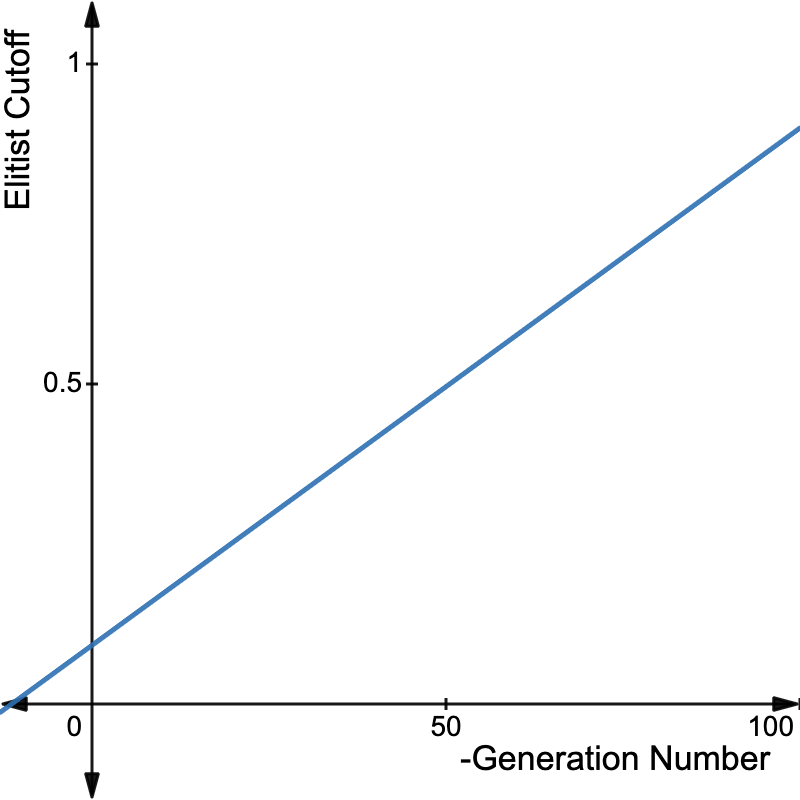
\includegraphics[width=0.34\textwidth]{Thesis/diagrams/cutoff-graph.png}
    \caption{Elitist cutoff by round for $l=100$}
    \label{fig:cutoff_graph}
\end{figure}

This is a technique used in many applications of GAs \cite{holland1992, larranaga1999}. The intuition is that it promotes initial genetic diversity while also allowing later generations to focus more on small-tweaks to the solution, rather than overhauling existing methods. This technique is analogous to a decaying learning rate in other fields in machine learning. 

\subsection{Zone Evaluator} 
An important factor absent from the previous model is how efficiently we connect people to their desired destination. This property is highly desirable in an effective transit system. A common approach to address this issue is to make use of a \textit{demand matrix} \cite{arbex2015, ceder2016, bielli2002}. A demand matrix is a concise representation for the demand for different kinds of point-to-point journeys. Most commonly, an entry $a_{ij}$ in a demand matrix $D$ represents the demand for journeys from point $i$ to point $j$. The size of such a matrix can vary greatly depending on how we define a \textit{point} for the context of the demand matrix. 

One approach is to define points as stops in the network, and have the demand matrix describe the desire to go from any stop to any other in the network. While such an approach is very powerful, it presents a few issues. First, the dimensions of such a matrix are $|S|\times|S|$ where $S$ is the set of stops, meaning that even in our simplified SFMTA network, this matrix has almost 300,000 entries. Thus, working with such a matrix is very computationally expensive. The second and more severe issue is that this data does not currently exist for large scale networks and would be incredibly difficult to estimate accurately. Thus, having to take on the computational burden of estimating and working with a large matrix, while not having high confidence in its exact values makes such an approach unrealistic. 

Therefore, as has been done throughout this project, we simplify the problem to a smaller scale, while attempting to maintain the benefits of its more complex representation. We define a \textit{Zone Evaluator} as a simple implementation of the demand matrix idea. Specifically, we define \textit{zones} of the city and use the zones instead of individual stops in our demand matrix. Thus, the dimensions of such a matrix are reduced to $|Z|\times|Z|$ where $Z$ is the set of zones. Each zone is defined as a point in longitude and latitude and covers the area within a radius of $\delta_{zone} = 900 m$. See Figure \ref{fig:zone-plot} for a representation of the chosen zones. 
\begin{figure}[h]
    \centering
    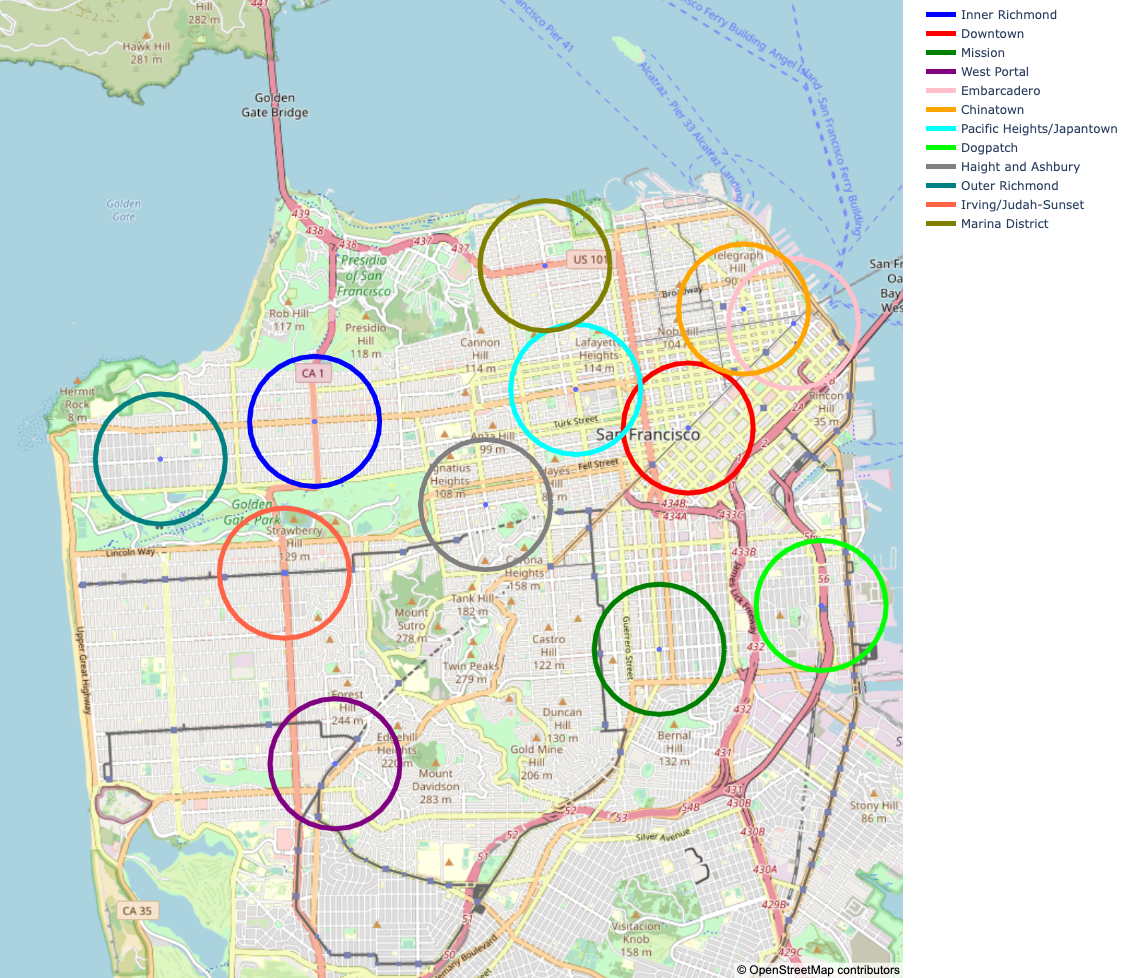
\includegraphics[width=\textwidth]{Thesis/diagrams/zone-plot.png}
    \caption{Plot of zones}
    \label{fig:zone-plot}
\end{figure}
With this configuration, we have a 12 by 12 demand matrix, which significantly simplifies any relevant computation. Each entry within this table represents the demand for a journey from one zone to another. Zones can be thought of high demand transit areas, and intuitively represent areas we want to reward our model for high transit activity and transfers. In order to set such entries, we use a very simple estimation method: all zones have a strong desire to get to downtown, and a less strong desire to get to other zones. More specialized methods of approximating the demand between zones is worth investigation and is a topic we will return to later. 

\subsection{Evaluating the Zone Score of a Network}
With the Zone Evaluator now defined, we must address how it can be used to evaluate a network's ability to connect different areas of the city together. We define the zone score of a network $z(n)$ as the weighted average \textit{stop-distance} between zones, where the weight for each pair of zones corresponds to the demand for that journey. To define how we compute this more precisely, let us start with some smaller sub-problems we make use of on our way up to defining the overall computation of zone score for a network. 

The simplest problem is the \textit{stop zone distance via route} problem. That is, how do we compute the distance from some stop $s$ to some zone $z$ along some route $r$, where distance is measured in stops along route $r$. When at the stop, we can choose to go in the trip in either direction to potentially reach our target zone $z$. This perspective is demonstrated in Figure \ref{fig:zone-distance}. 

\begin{figure}[H]
    \centering
    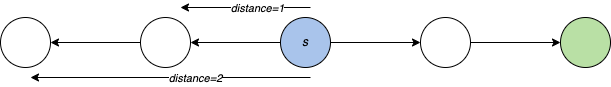
\includegraphics[width=\textwidth]{Thesis/diagrams/stop-zone-distance.png}
    \caption{Single route view with a stop in the blue zone and another stop on the route in the green zone.}
    \label{fig:zone-distance}
\end{figure}
Suppose we are at stop $s$ and our goal is to measure our distance to the green zone. To do so, we perform a single dimensional breadth-first-search on this graph representation to find the direction that minimizes the number of stops to the green zone. If we reach the end of the route in both directions, we give the distance a default $\delta_{default}= 90$ stops to punish non-connected zones. 

Now, we can look at the \textit{stop zone distance} across all routes at some stop $s$ to some zone $z$. Let $Rt$ be the set of routes that transfer at stop $s$. Then, for each $r \in Rt$ we compute the stop zone distance of stop $s$ via route $r$ to $z$, and take the minimum across all $r \in Rt$ as our overall stop zone distance. 

We can now define the overarching problem of computing the stop distance between zones. For a given pair of zones $z_1$ and $z_2$, we uniformly sample $k_{s}$ \textit{source stops} from $z_1$ without replacement, where $k_{s}$ is some hyper-parameter currently defaulted to $5$. For each stop we sample, we compute the stop zone distance from the stop in $z_1$ to $z_2$, then take the average across all samples as our zone distance score $z(n)$. Similar to all other metrics discussed, we re-scale $z(n)$ to $Z(n)$: a value relative to the score for the original network. 

There are few important subtle details here to note. First, the randomly sampled stops for a given zone are fixed for each generation of the model. That is, before evaluating a population, we sample our $k_s$ stops for each zone and keep them fixed for each zone evaluation score generated on this generation. In other words, within a given generation, the evaluation is done using the same stops as the source stops of each zone. Secondly, notice that we have introduced some randomness into our network evaluation, whereas before it was completely deterministic. This randomness has the potential to introduce noise in the fitness, which we attempt to minimize by sampling multiple stops within the zone and averaging the results. Finally, we do not allow transferred connections between zones. If no direct connection exists, we default the zone distance to $\delta_{default}$. The decision to not allow for transfers places an emphasis on direct routes between zones. This is in line with the intuition of zones as transit hubs or popular transfer destination. That is, in a system with connections between all zones, any trip can be achieved by accessing the nearest zone, then transferring from there. 

\subsection{New Fitness Function}
With new metrics comes a new fitness function. Based on the initial results in Section 4, the metrics for coverage, ridership, and number of routes have all been excluded from the new iteration of the fitness function. Coverage and ridership were excluded because their values appeared to be preserved by the fitness function. Additionally, the number of routes as a metric was excluded because it grew linearly with generations regardless of how the networks were structured, making it a poor indicator of an effective network. 

In their place, we have our two new metrics: extreme trip score $E(n)$, and zone evaluator score $Z(n)$. Together, this redefines our fitness function:
\begin{align*}
    F(n) = \frac{(\lambda_{E} E(n) + \lambda_{Z} Z(n) +\lambda_{D} D(n))}{(\lambda_{E} + \lambda_{Z} + \lambda_{D})}.
\end{align*}
\section{New Algorithm Results} 
\subsection{Experimenting with Fitness Function Weights}
To develop a deeper understanding of the model and specifically its new fitness function, experimenting with many different values for the $\lambda$ weights serves as a natural first step. The model was batch run with $11$ different choices of the $\lambda$ hyper-parameters depicted in Table \ref{table:batch-run-configs}.

\begin{figure}[h]
    \centering
    \begin{tabular}{|c|c|c|c|}
        \hline
        Config. \# & $\lambda_D$ & $\lambda_Z$ & $\lambda_E$ \\
         \hline
        1 & 2 & 2 & 1 \\
        2 & 2 & 4 & 1 \\
        3 & 4 & 2 & 1 \\ 
        4 & 3 & 3 & 1 \\ 
        5 & 6 & 3 & 1 \\ 
        6 & 3 & 6 & 1 \\ 
        7 & 1 & 1 & 1 \\
        8 & 1 & 10 & 1 \\ 
        9 & 10 & 1 & 1 \\
        10 & 0 & 1 & 0 \\ 
        11 & 1 & 1 & 0 \\
        \hline
    \end{tabular}
    \caption{Tested configurations of $\lambda$ hyper-parameters}
    \label{table:batch-run-configs}
\end{figure}

Each run of the model was done for 200 generations and with a population size of 100. The zone evaluation step in the new version of the model introduces a much longer computation, making it unrealistic to use a population size of $N=1000$, as was done with the initial model, in a reasonable amount of time.\footnote{This was an overnight batch run on the order of 10-11 hours to complete all of the runs, which was deemed on the border of reasonable.} Note that the configurations of the hyper-parameters tested is based on smaller-scale testing, as well as being partly arbitrary. 

To begin, consider a configuration of the weights that did not produce meaningful results. When running the model with configuration $11$, the one without incorporating the extreme trip score, we see similar results to the first iteration of the model. The fitness sky-rockets (see Figure \ref{fig:no-extreme-trips}), but upon examination of the networks, the issue of super-routes is still present.\footnote{Note that most of the sub-scores are not visible, since the scale causes them all to be on top of each other at 0.}

\begin{figure}[H]
    \centering
    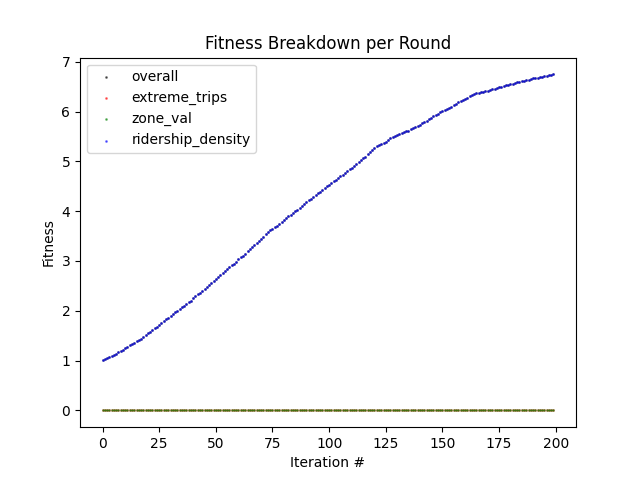
\includegraphics[width=\textwidth]{Thesis/diagrams/second_run/fitness_breakdown(110).png}
    \caption{Average fitness sub-scores by generation with no extreme trip punishment}
    \label{fig:no-extreme-trips}
\end{figure}

Notice that the fitness becomes fully determined by the ridership density metric and it drowns out the effect of the zone score. This suggests that it is specifically the ridership density that benefits from creating unrealistically long, and potentially short routes. Since ridership density rewards transfer points on high ridership lines, the model converges toward networks with the routes that are the longest, highest ridership, and contain the most number of transfer points. 

However, when we include the extreme trips metric, the same effect does not occur, indicating that this new metric is successful in limiting the ridership density from abusing unrealistic trip constructions to achieve higher fitness scores. For an example refer to Figure \ref{fig:631-plot}.

\begin{figure}[h]
    \centering
    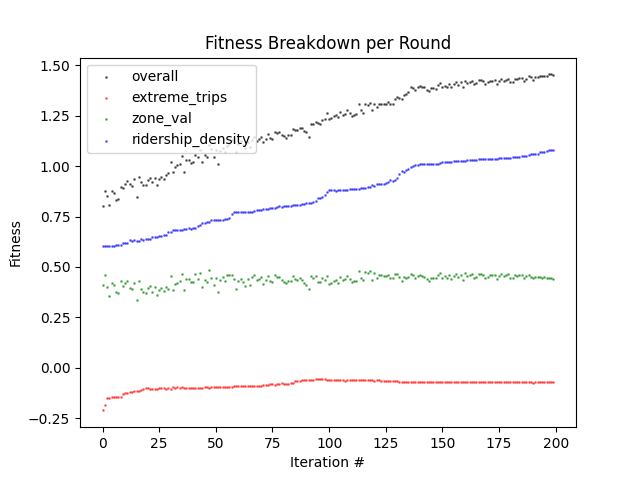
\includegraphics[width=\textwidth]{Thesis/diagrams/second_run/fitness_breakdown(631).png}
    \caption{Configuration \# 6 fitness breakdown}
    \label{fig:631-plot}
\end{figure}

In fact, configuration 6 (seen in Figure \ref{fig:631-plot}) achieved the most promising results across the trials for a few reasons. First, the fitness function appears to incorporate all metrics in the calculation. Secondly, the fitness of the model begins to level off, toward later generations (see Figure \ref {fig:631-plot-trend}), suggesting that the algorithm is beginning to converge. 

\begin{figure}[H]
    \centering
    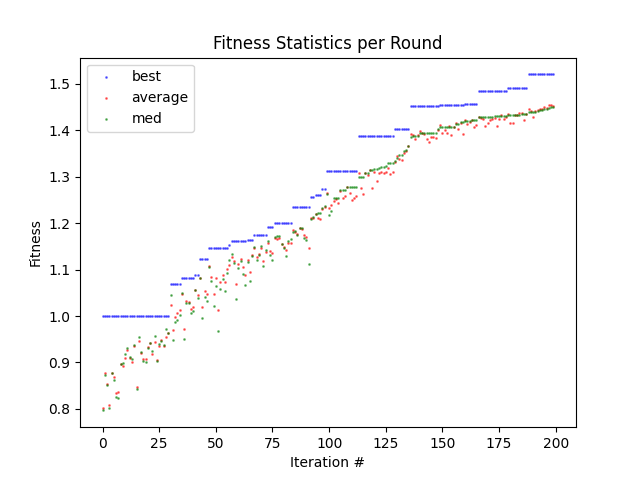
\includegraphics[width=\textwidth]{Thesis/diagrams/second_run/fitness_trend(631).png}
    \caption{Configuration \# 6: fitness trend}
    \label{fig:631-plot-trend}
\end{figure}

In addition to displaying behavior expected from a strong GA, this run also exhibits many of the trends seen in some runs for other $\lambda$ weightings. Notable among these trends is the tendency for the extreme trip score, as well as the zone score, to converge to some bound before leveling off, while the ridership density score is able to grow, but at a decreasing rate. This pattern highlights a potential flaw in that the zone distance score is unable to improve to the point of contributing significant fitness. 

A possible explanation for this shortcoming is that the SFMTA original system is already designed in such a way that highly optimizes this zoning approach. First, recall that in the zoning evaluation, we gave more weight to the trips to and from downtown. SFMTA designed their network such that each major area has at least one line directly to downtown, meaning that the zone distance score cannot be improved. 

Another trend worth discussion is the reduction of noise in the zone distance score of the population seen in Figure \ref{fig:631-plot}. In early generations, this value moves slightly, likely due to noise from sampling random stops each generation. However, this noise decreases significantly as the generations increase. This suggests that regardless of the random samples, the networks are producing similar zone distance scores. Such a habit could be explained by networks creating multiple routes in between each zone, such that regardless of which stops are sampled, the zone evaluator finds a trip reaching the target zone. This explanation is further supported in the following section where we examine the best performing network. 

\subsection{Examining best performing networks}
In this section, we will continue with configuration \#6. Looking at the best performing network of the final generation for this run of the model, many interesting patterns come to light. While the overall structure is very similar to the original network, compare Figures \ref{fig:original-no-stops} and \ref{fig:6bestperformer-no-stops}, the underlying route geometry has changed significantly. 

\begin{figure}
\centering
\begin{minipage}{.5\textwidth}
  \centering
  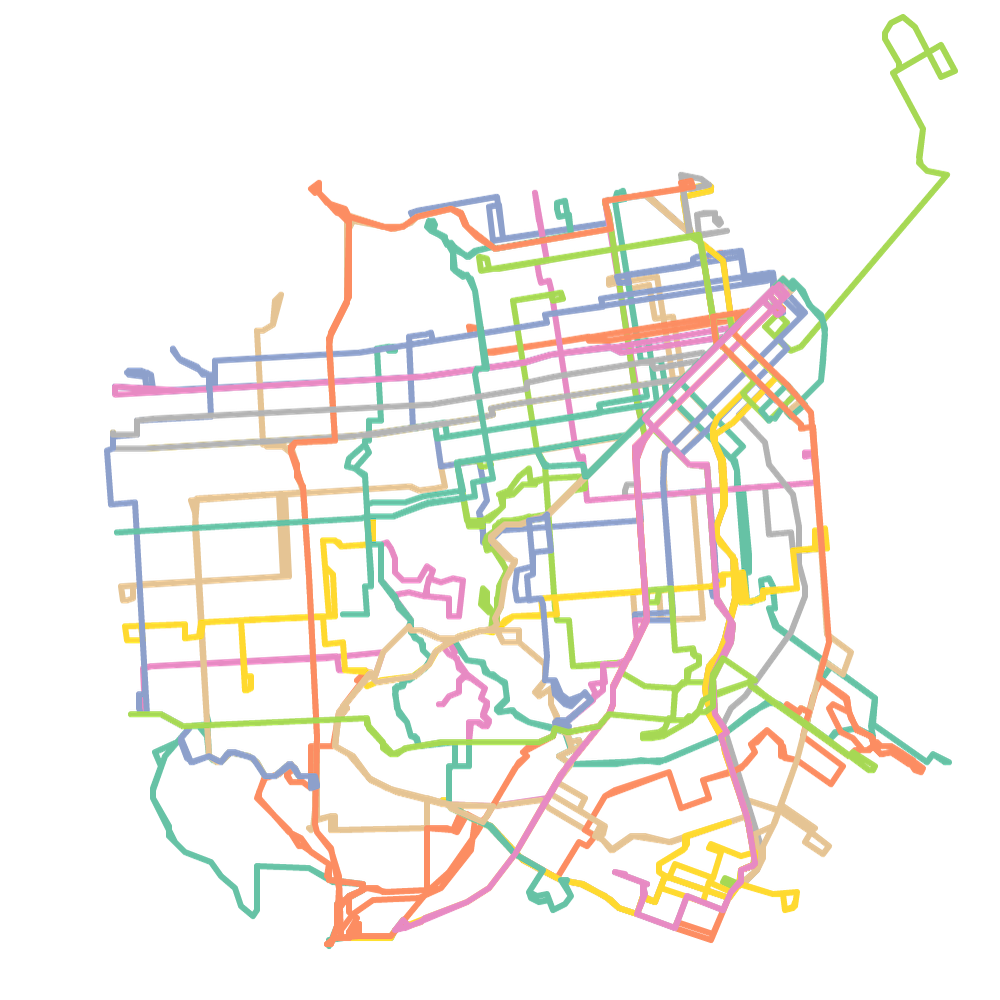
\includegraphics[width=\linewidth]{Thesis/diagrams/original-no-stops.png}
  \caption{Original network without stops marked}
  \label{fig:original-no-stops}
\end{minipage}%
\begin{minipage}{.5\textwidth}
  \centering
  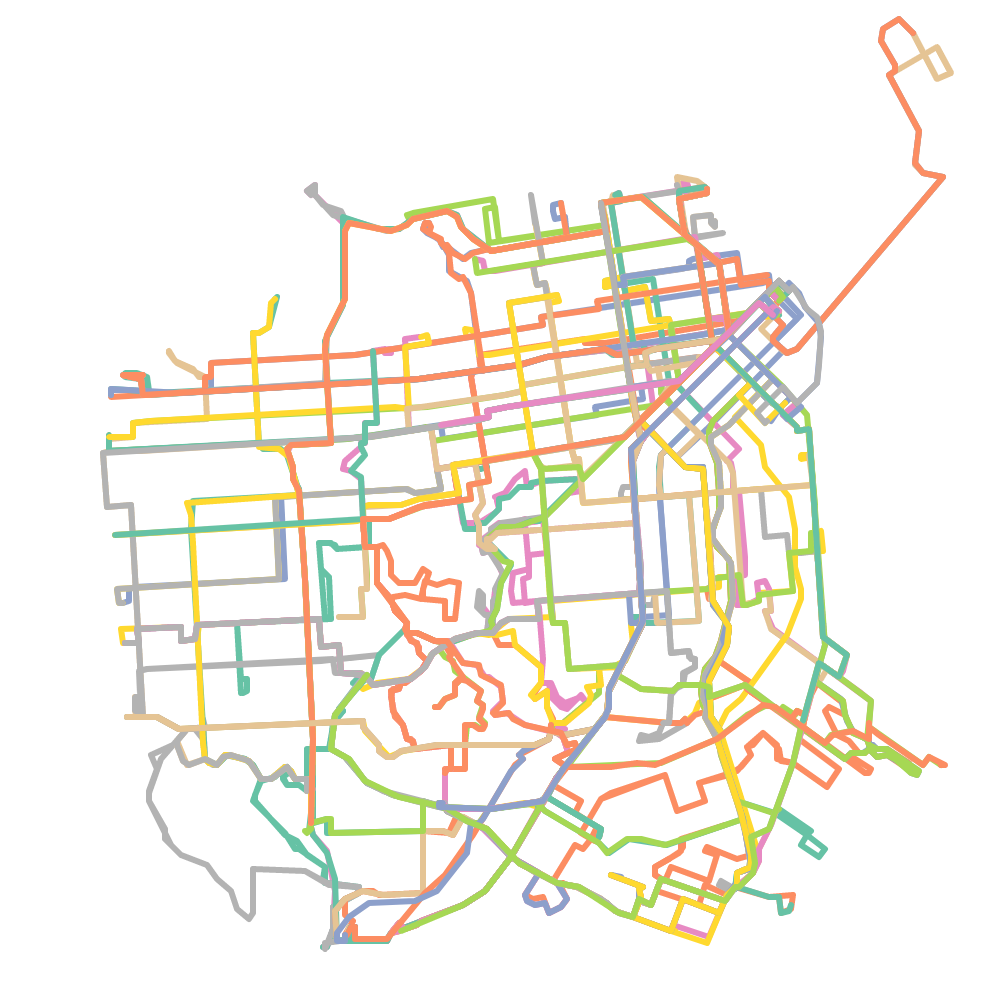
\includegraphics[width=\linewidth]{Thesis/diagrams/second_run/best-performer-no-stops.png}
  \caption{Configuration \# 6 best performer without stops marked.}
  \label{fig:6bestperformer-no-stops}
\end{minipage}
\end{figure}

Specifically, a large majority of the new routes, routes created from SPCrossover, go through downtown. See Figure \ref{fig:downtown-routes} for a sample of some of these routes. 

\begin{figure}
    \centering
    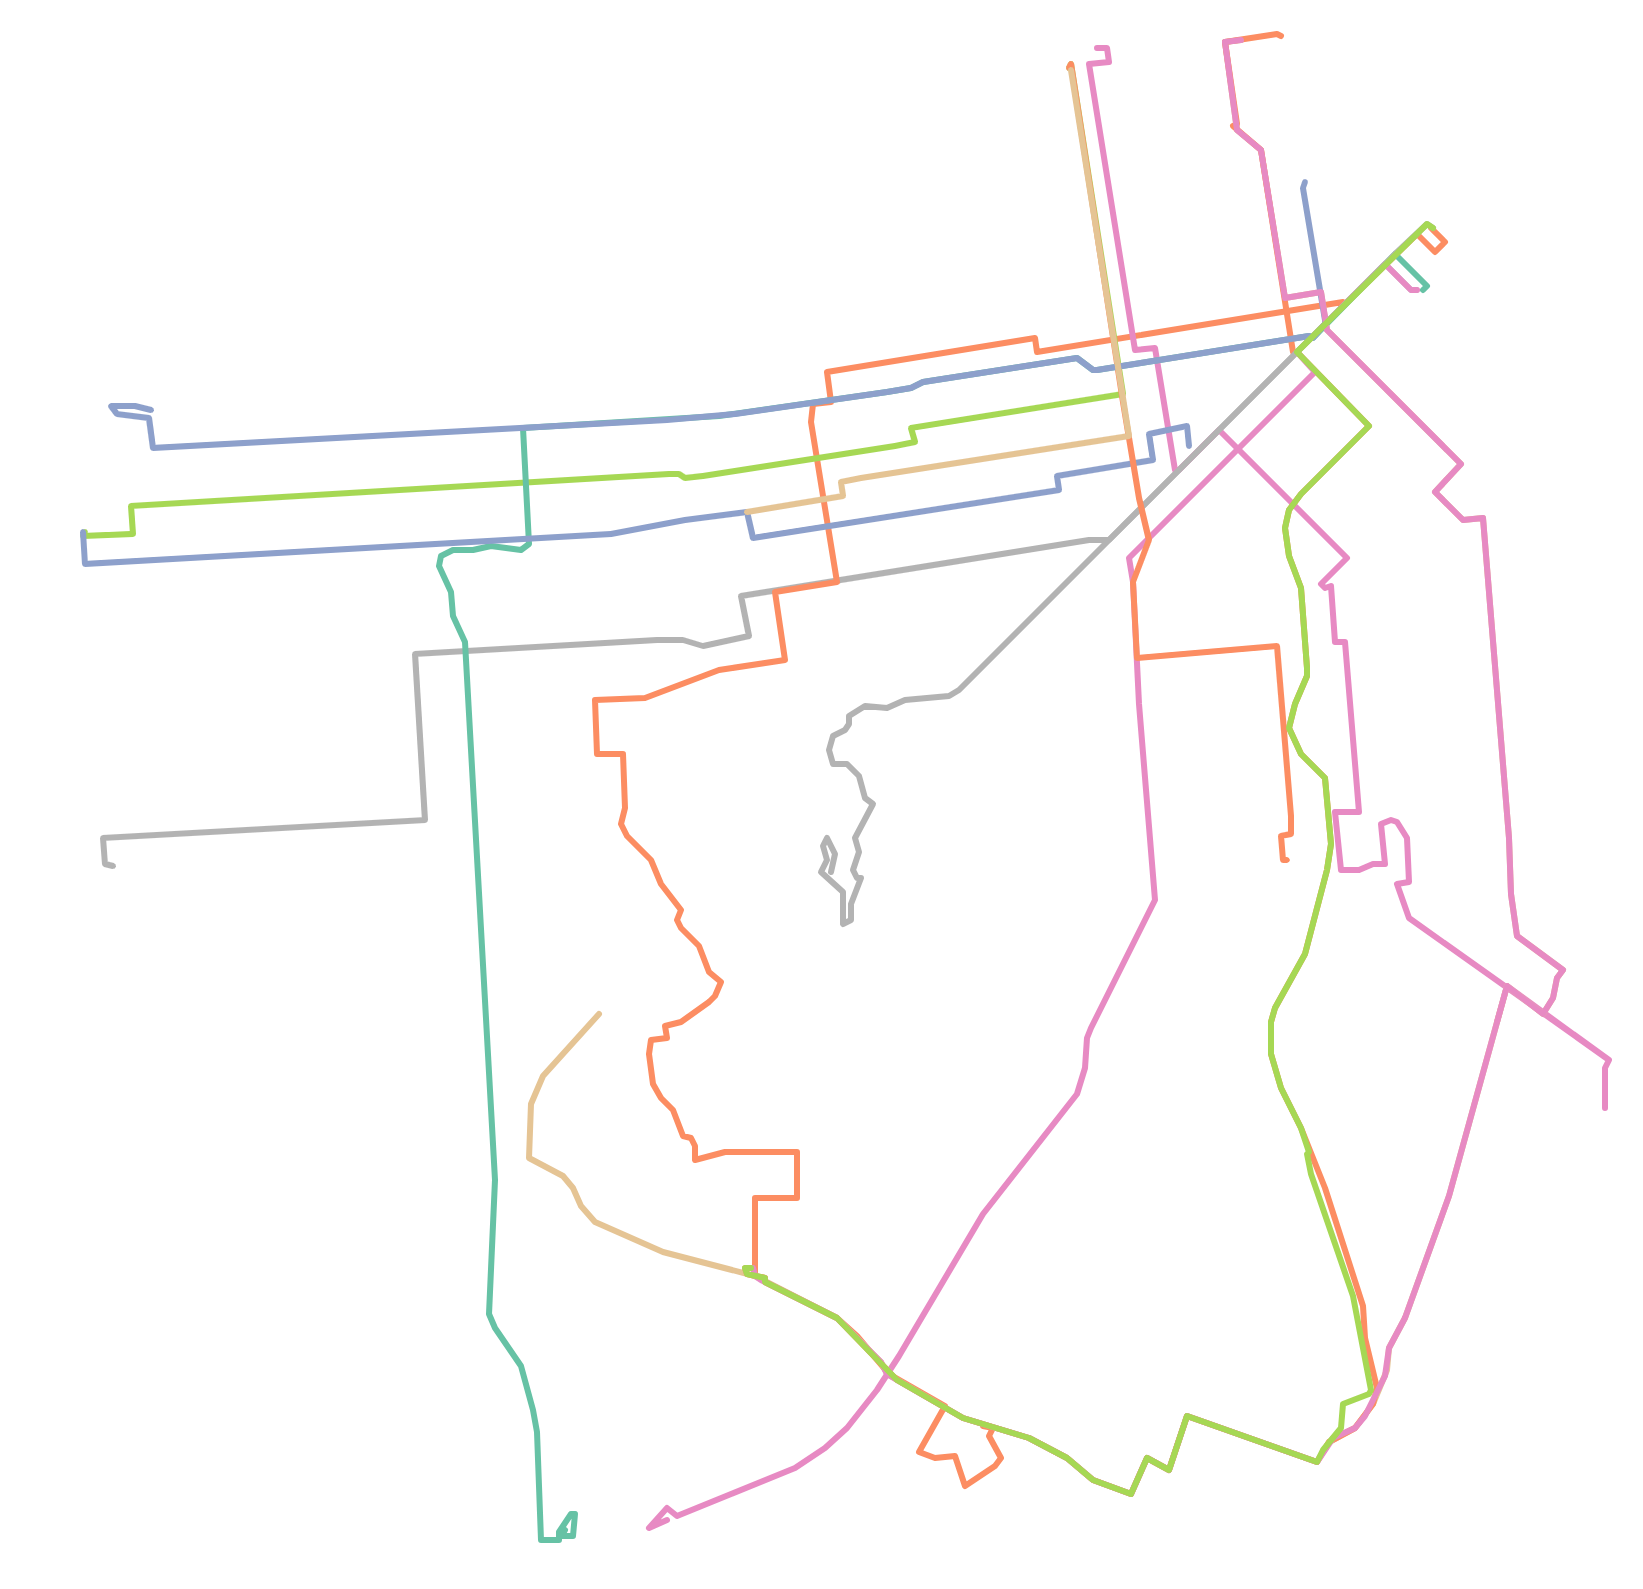
\includegraphics[width=0.5\textwidth]{Thesis/diagrams/second_run/new-downtown-routes.png}
    \caption{Sample of routes created by SPCrossover in best performer of configuaration \# 6}
    \label{fig:downtown-routes}
\end{figure}

There are two possible explanations for why this is occurring: an optimistic one and a pessimistic one. In the optimistic view, this is due to how our model highly rewards direct routes to downtown via the zone evaluation metric in the fitness function. Additionally, rewarding ridership density encourages the model to have a higher number of routes downtown, where there are more transfers. 

In contrast, the pessimistic view suggests this is simply be explained by the fact that most routes originally go through downtown, and therefore when we randomly sample transfer points for breeding, we are likely to sample ones in the downtown area, making sure the route still stops downtown. Notice that in SPCrossover, whichever transfer point we sample will be a stop on both of the child trips. Thus, if we sample a transfer stop downtown,  both child trips are guaranteed to contain a stop in the downtown area. 

However, there a few pieces of evidence to support the optimistic view. First, the proportion of routes downtown in the breeded routes far surpasses that in the original network. Thus, the model must be rewarding networks with more routes downtown in some fashion. Additionally, the shape of such routes does not appear to be randomly sprawling out from downtown, but rather connecting downtown to a specific zone. Examining Figure \ref{fig:downtown-routes} and \ref{fig:zone-plot} together shows that the routes branching off of downtown often branch directly to a zone. For example, consider the grey route in Figure \ref{fig:downtown-routes} that connects the far left side of the city to downtown. Looking at this route in the context of the zone diagram of \ref{fig:zone-plot} we notice that it directly connects to the Irving-Judah-Sunset zone and passes through the Haight and Ashbury zone. Thus, this route likely allows for efficient trips between the three zones along its line, resulting in a higher zone score of the overall network. 

Overall, the high concentration of routes in the downtown area reflects our model's bias towards ridership over coverage. This bias is apparent in the fitness function as we removed the metric that was used to track it. Recall that the reason for removing this metric was because it was assumed to stay constant across the SPCrossover. However, it is equally possible the flaw was in methods of measuring coverage itself, and perhaps a more nuanced approach to measuring coverage in the transit network is needed. 

\section{Future Work}
So far, the exploration has focused on the changing of weights in the fitness function. However, the analysis need not stop there. Some other aspects of the model worth investigation involve the fitness function itself, and potentially opening the door to non-linear combinations of factors. In addition to a non-linear fitness function, further exploration of other potential metrics is needed. There are many important qualities of transit networks not captured in this model for optimizing geometry of networks, such as efficient transfer usage, and placing transit hubs effectively. 

Additionally, there is a core idea in genetic algorithms currently missing in the implementation of this model: mutation. Mutation is traditionally applied as the random flip of a bit or change of a single value. However, in the context of this project, we are not using a binary encoding, meaning that this idea can not be directly applied. Instead, the intuition behind flipping a random bit in an binary encoding would have to be adapted to the context of working with transit networks as a whole. Among the ideas considered to adapt this idea within this project were: randomly deleting routes from a network, randomly splitting or combining routes within a network, and randomly adding a route to some network from another in the population. However, each presents its own unique set of challenges in practice. Specifically, none of these mutations appear natural to the problem of route design as randomly dropping or randomly splitting routes doesn't appear beneficial in the process of designing a network. Ideally, each route should be part of a system of routes that work together to connect different areas of the city. 

In terms of extensions to the existing model, there are a few areas worth highlighting. First, the zone evaluator currently uses a very simple heuristic to determine the desire for a specific journey from one zone to another. A better approach would likely be to incorporate the existing ridership data as a means of estimating the existing desire to get from one zone to another. 

Additionally, the mapping of the zones themselves is arbitrary, as it is based on areas that tend to have many transit stops and also serve as likely destinations for a trip. As an improvement, one could apply clustering algorithms, such as $k$-means clustering, to population density data to automatically generate zones in the city based on population density. That is, if we plot the population of the city as points in space over the map of the city, where each point represents some fixed number of people living in some location, running a clustering algorithm on such points would generate zones based on the population density itself. Such zones would likely serve as stronger candidates for the zone evaluator used in the model. 

Second, working with the networks directly throughout the model becomes both computationally demanding and increasingly restrictive. Perhaps a clever encoding scheme for an entire network could be realized that preserves the natural hierarchy of the routes, trips, and stops. With such a representation, the crossover and mutation operations would follow more naturally, assuming the encoding was structured in such a way that all encoding corresponded to viable networks. 

Third, the project only considers the bus network of SFMTA and ignores the expanding subway network, as well as the street-cars and ferries in use. A natural way to extend to incorporate other methods of transportation would be add a constraint to routes that can be bred, in that they must also be the same method of transportation, that is bus routes only with bus routes and street-car routes only with street-car routes and so on.   

A final extension worth mention is that all of the code developed for this project, with the exception of the specification of the zones themselves, was not specific to running on San Francisco's transit system. In fact, this can be run on any transit system with a GTFS specification, and the corresponding ridership data. Currently, ridership data has alreadly been obtained from other agencies such as SEPTA(Southeastern Pennsylvania Transportation Authority), that could be used to run the same experiments.\footnote{SFMTA was chosen as the main network to experiment with due to its smaller size, and my overall familiarity with both the system and the city. SEPTA is order of magnitudes larger, and therefore presents increased computational burden and complications.} By running the model on multiple cities, one could compare the results across them to generate more general trends, as its possible the results of the model on the SFMTA network were partly due to design decisions in the SFMTA network. Running the model on SEPTA data, and other transit agencies would not only allow us to confirm such a hypothesis, but also highlight which elements of the results are dependent on the original network design, and which are intrinsic to the model itself. 

\section{Conclusion}
In conclusion, a major result of this project is the demonstration of the sensitivity of the genetic algorithm fitness function. That is, because the genetic algorithm is randomly searching some space of solutions with the fitness function as a guide, any details in the fitness function the algorithm can abuse to achieve higher fitness, will be abused. In both iterations of the model we saw such behavior. First, the original model produced super routes to maximize fitness when no constraint was placed on trip length. Then, with the new zone evaluator feature, the model produced routes almost exclusively downtown to maximize ridership density, while also connecting each zone to the downtown area, a behavior highly rewarded in the fitness function. 

In addition, the problem of optimizing the geometry of routes has shown to be incredibly complex. Specifically, the ability to evaluate many different geometries, and determine which is best, is a difficult task with many potential approaches. In general, the problem also proves to be computationally demanding, suggesting that fully automating the entire process may produce diminishing returns on computing power in comparison to hybrid approaches including both manual and automatic optimization techniques. The ultimate goal of improving public transit improvement requires both the computational tools, but also the personal experience to identify what the important factors are \cite{fitzgerald2022}. As demonstrated in this project, each time we changed the fitness function, another piece of the system fell out of balance. First, it was the length of the routes, then it was the over-concentration of routes to the downtown area. Such behavior reinforces the ideas discussed in the introduction of transit optimization about the difficulty of maximizing multiple objectives at the same time, especially when their success is competing. Specifically, more nuance and care is needed in the design of transit systems to see how seemingly contradicting objectives, such as ridership and coverage, can be realized in an actual system. 
\section*{Acknowledgements}
I first want to thank my advisor Robert Manning for the consistent feedback provided throughout the entire process, as well as giving me the freedom to explore topics that interested me. I also want to thank SFMTA and SEPTA for providing the data that fueled my analysis. 
\section*{Appendix}
Source code for this project can be found at: \url{https://github.com/Hweinstock/TransitGA}.

\printbibliography
\end{document}

